%% Copyright 2021, Eliska Sestakova and Ondrej Guth
%%
%% This work may be distributed and/or modified under the
%% conditions of the LaTeX Project Public Licenese, either version 1.3
%% of this license or (at your option) any later version.
%% The latest version of this license is in
%%  https://www.latex-project.org/lppl.txt
%% and version 1.3 or later is part of all distributions of LaTeX
%% version 2005/12/01 or later.
%%
%% This work has the LPPL maintenance status `maintained'.
%%
%% The current maintainer of this work is Ondrej Guth.
%% Contact ondrej.guth@fit.cvut.cz for bug reports.
%% Alternatively, submit bug reports into the tracker at
%% https://gitlab.fit.cvut.cz/theses-templates/FITthesis-LaTeX/issues
%%
%%

%%%%%%%%%%%%%%%%%%%%%%%%%%%%%%%%%%%%%%%%%
% CLASS OPTIONS
% language: czech/english/slovak
% thesis type: bachelor/master/dissertation
%%%%%%%%%%%%%%%%%%%%%%%%%%%%%%%%%%%%%%%%%
\PassOptionsToPackage{dvipsnames}{xcolor}

\documentclass[czech,master,unicode]{ctufit-thesis}

%%%%%%%%%%%%%%%%%%%%%%%%%%%%%%%%%%
% FILL IN THIS INFORMATION
%%%%%%%%%%%%%%%%%%%%%%%%%%%%%%%%%%
\ctufittitle{Mobilní aplikace pro zobrazení výsledků hlasování Poslanecké sněmovny}

\ctufitauthorfull{Bc. Lukáš Dang}

\ctufitauthorsurnames{Dang}

\ctufitauthorgivennames{Lukáš}

\ctufitsupervisor{Ing. Ondřej John}

\ctufitdepartment{Katedra webového inženýrství} % 

\ctufityear{2023}

\ctufitdeclarationplace{Praze}

\ctufitdeclarationdate{\today}

\ctufitabstractCZE{Diplomová práce popisuje návrh a implementaci mobilní aplikace, která slouží k zobrazení výsledků hlasování poslanců Poslanecké sněmovny Parlementu ČR. Součástí práce je i návrh \linebreak a implementace backendu, který bude zpracovávat data z webu poslanecké sněmovny parlamentu ČR a poskytovat je mobilní aplikaci prostřednictvím REST API.}
	
\ctufitabstractENG{The diploma thesis describes the design and implementation of a mobile application that serves to display the voting results of members	 of the Czech Parliament's Chamber of Deputies. The work also includes the design and implementation of a backend that will process data from the Czech Parliament's Chamber of Deputies website and provide it to the mobile application through \linebreak a REST API.}

\ctufitkeywordsCZE{poslanecká sněmovna, parlament, hlasování, poslanec, poslanecký klub, REST, Android, mobilní aplikace, backend, Kotlin, Java}

\ctufitkeywordsENG{Chamber of Deputies, parliament, voting, member of parliament, parliamentary party group, REST, Android, mobile application, backend, Kotlin, Java}

\RequirePackage{iftex}[2020/03/06]
\iftutex % XeLaTeX and LuaLaTeX
    \RequirePackage{ellipsis}[2020/05/22] %ellipsis workaround for XeLaTeX
\else
    \RequirePackage[utf8]{inputenc}[2018/08/11] %this file encoding
    \RequirePackage{lmodern}[2009/10/30] % vector flavor of Computer Modern font
\fi

% hyperlinks
\RequirePackage[pdfpagelayout=TwoPageRight,colorlinks=false,allcolors=decoration,pdfborder={0 0 0.1}]{hyperref}[2020-05-15]

% uncomment the following to hide all hyperlinks
% \RequirePackage[pdfpagelayout=TwoPageRight,hidelinks]{hyperref}[2020-05-15]

\RequirePackage{pdfpages}[2020/01/28]

\setcounter{secnumdepth}{4} % numbering sections; 4: subsubsection

\usepackage[T1]{fontenc}
\usepackage{float}

\newcommand{\imagepath}{images}

\usepackage{graphicx}
\usepackage{subcaption}
\graphicspath{ {images/} }

\colorlet{punct}{red!60!black}
\definecolor{background}{HTML}{EEEEEE}
\definecolor{delim}{RGB}{20,105,176}
\colorlet{numb}{magenta!60!black}

\usepackage{dirtree}
\usepackage{lipsum,tikz}
\usepackage{csquotes}
\usepackage[style=iso-numeric]{biblatex}
\usepackage{listings} % typesetting of sources

\addbibresource{text/bib-database.bib}

\lstset
{ %Formatting for code in appendix
	language=Matlab,
	basicstyle=\footnotesize,
	numbers=left,
	stepnumber=1,
	showstringspaces=false,
	tabsize=1,
	breaklines=true,
	breakatwhitespace=false,
}

\lstdefinelanguage{Kotlin}{
	comment=[l]{//},
	commentstyle={\color{gray}\ttfamily},
	emph={filter, first, firstOrNull, forEach, lazy, map, mapNotNull, println},
	emphstyle={\color{OrangeRed}},
	identifierstyle=\color{black},
	keywords={!in, !is, abstract, actual, annotation, as, as?, break, by, catch, class, companion, const, constructor, continue, crossinline, data, delegate, do, dynamic, else, enum, expect, external, false, field, file, final, finally, for, fun, get, if, import, in, infix, init, inline, inner, interface, internal, is, lateinit, noinline, null, object, open, operator, out, override, package, param, private, property, protected, public, receiveris, reified, return, return@, sealed, set, setparam, super, suspend, tailrec, this, throw, true, try, typealias, typeof, val, var, vararg, when, where, while},
	keywordstyle={\color{NavyBlue}\bfseries},
	morecomment=[s]{/*}{*/},
	morestring=[b]",
	morestring=[s]{"""*}{*"""},
	ndkeywords={@Deprecated, @JvmField, @JvmName, @JvmOverloads, @JvmStatic, @JvmSynthetic, Array, Byte, Double, Float, Int, Integer, Iterable, Long, Runnable, Short, String, Any, Unit, Nothing},
	ndkeywordstyle={\color{BurntOrange}\bfseries},
	sensitive=true,
	stringstyle={\color{ForestGreen}\ttfamily},
}

\lstdefinelanguage{json}{
	basicstyle=\normalfont\ttfamily,
	numbers=left,
	numberstyle=\scriptsize,
	stepnumber=1,
	numbersep=8pt,
	showstringspaces=false,
	breaklines=true,
	frame=lines,
	backgroundcolor=\color{background},
	literate=
	*{0}{{{\color{numb}0}}}{1}
	{1}{{{\color{numb}1}}}{1}
	{2}{{{\color{numb}2}}}{1}
	{3}{{{\color{numb}3}}}{1}
	{4}{{{\color{numb}4}}}{1}
	{5}{{{\color{numb}5}}}{1}
	{6}{{{\color{numb}6}}}{1}
	{7}{{{\color{numb}7}}}{1}
	{8}{{{\color{numb}8}}}{1}
	{9}{{{\color{numb}9}}}{1}
	{:}{{{\color{punct}{:}}}}{1}
	{,}{{{\color{punct}{,}}}}{1}
	{\{}{{{\color{delim}{\{}}}}{1}
	{\}}{{{\color{delim}{\}}}}}{1}
	{[}{{{\color{delim}{[}}}}{1}
	{]}{{{\color{delim}{]}}}}{1},
}

% \usepackage{minted} % typesetting of sources
\usepackage{longtable}

%theorems, definitions, etc.
\theoremstyle{plain}
\newtheorem{theorem}{Věta}
\newtheorem{lemma}[theorem]{Tvrzení}
\newtheorem{corollary}[theorem]{Důsledek}
\newtheorem{proposition}[theorem]{Návrh}
\newtheorem{definition}[theorem]{Definice}
\theoremstyle{definition}
\newtheorem{example}[theorem]{Příklad}
\theoremstyle{remark}
\newtheorem{note}[theorem]{Poznámka}
\newtheorem*{note*}{Poznámka}
\newtheorem{remark}[theorem]{Pozorování}
\newtheorem*{remark*}{Pozorování}
\numberwithin{theorem}{chapter}
%theorems, definitions, etc. END
%%%%%%%%%%%%%%%%%%%%%%
% DEMO CONTENTS SETTINGS END
%%%%%%%%%%%%%%%%%%%%%%

\begin{document} 
\frontmatter\frontmatterinit % do not remove these two commands


\includepdf{assignment-include.pdf} % replace that file with your thesis assignment provided by study office

\thispagestyle{empty}\cleardoublepage\maketitle % do not remove these three commands

\imprintpage % do not remove this command

\tableofcontents % do not remove this command
%%%%%%%%%%%%%%%%%%%%%%
% list of other contents: figures, tables, code listings, algorithms, etc.
% add/remove commands accordingly
%%%%%%%%%%%%%%%%%%%%%%
\listoffigures % list of figures
\begingroup
\let\clearpage\relax
\listoftables % list of tables
\lstlistoflistings % list of source code listings generated by the listings package
% \listoflistings % list of source code listings generated by the minted package
\endgroup
%%%%%%%%%%%%%%%%%%%%%%
% list of other contents END
%%%%%%%%%%%%%%%%%%%%%%

%%%%%%%%%%%%%%%%%%%
% ACKNOWLEDGMENT
% FILL IN / MODIFY
% This is a place to thank people for helping you. It is common to thank your supervisor.
%%%%%%%%%%%%%%%%%%%
\begin{acknowledgmentpage}
	Rád bych tímto poděkoval svému vedoucímu, Ing. Ondřej John, za jeho vstřícnost, trpělivost a čas, který mi věnoval při vedení mé diplomové práce. Dále bych chtěl poděkovat své rodině, která mě při psaní podporovala.
\end{acknowledgmentpage} 
%%%%%%%%%%%%%%%%%%%
% ACKNOWLEDGMENT END
%%%%%%%%%%%%%%%%%%%


%%%%%%%%%%%%%%%%%%%
% DECLARATION
% FILL IN / MODIFY
%%%%%%%%%%%%%%%%%%%
% INSTRUCTIONS
% ENG: choose one of approved texts of the declaration. DO NOT CREATE YOUR OWN. Find the approved texts at https://courses.fit.cvut.cz/SFE/download/index.html#_documents (document Declaration for FT in English)
% CZE/SLO: Vyberte jedno z fakultou schvalenych prohlaseni. NEVKLADEJTE VLASTNI TEXT. Schvalena prohlaseni najdete zde: https://courses.fit.cvut.cz/SZZ/dokumenty/index.html#_dokumenty (prohlášení do ZP)
\begin{declarationpage}
Prohla\v suji, \v ze jsem p\v redlo\v zenou pr\'aci vypracoval samostatn\v e a \v ze jsem uvedl ve\v sker\'e
pou\v zit\'e informa\v cn\'\i{} zdroje v~souladu s~Metodick\'ym pokynem o~do\-dr\v zo\-v\'an\'\i{} etick\'ych
princip\accent23u p\v ri p\v r\'\i{}prav\v e vysoko\v skolsk\'ych z\'av\v ere\v cn\'ych prac\'\i{}.

Beru na v\v edom\'\i{}, \v ze se na moji pr\'aci vztahuj\'\i{} pr\'ava a povinnosti vy\-pl\'y\-va\-j\'\i{}c\'\i{} ze z\'akona
\v c.\,121/2000~Sb., autorsk\'eho z\'akona, ve zn\v en\'\i{} pozd\v ej\v s\'\i{}ch p\v redpis\accent23u. V~souladu s~ust.\,\S{}\,2373 odst.\,2 z\'akona \v c.\,89/2012~Sb., ob\v cansk\'y z\'akon\'\i{}k, ve zn\v en\'\i{} pozd\v ej\v s\'\i{}ch p\v redpis\accent23u,
t\'\i{}mto ud\v eluji nev\'yhradn\'\i{} opr\'avn\v en\'\i{} (licenci) k~u\v zit\'\i{} t\'eto moj\'\i{} pr\'ace, a to v\v cetn\v e v\v sech
po\v c\'\i{}ta\v cov\'ych program\accent23u, je\v z jsou jej\'\i{} sou\v c\'ast\'\i{} \v ci p\v r\'\i{}lohou a ve\v sker\'e jejich
dokumentace (d\'ale souhrnn\v e jen \uv{D\'\i{}lo}), a to v\v sem osob\'am, kter\'e si p\v rej\'\i{} D\'\i{}lo u\v z\'\i{}t.
Tyto osoby jsou opr\'avn\v eny D\'\i{}lo u\v z\'\i{}t jak\'ymkoli zp\accent23usobem, kter\'y nesni\v zuje hodnotu
D\'\i{}la a za jak\'ymkoli \'u\v celem (v\v cetn\v e u\v zit\'\i{} k~v\'yd\v ele\v cn\'ym \'u\v cel\accent23um). Toto opr\'avn\v en\'\i{} je
\v casov\v e, teritori\'aln\v e i mno\v zstevn\v e neomezen\'e. 

\end{declarationpage}
%%%%%%%%%%%%%%%%%%%
% DECLARATION END
%%%%%%%%%%%%%%%%%%%

\printabstractpage % do not remove this command

%%%%%%%%%%%%%%%%%%%
% SUMMARY
% FILL IN / MODIFY
% OR REMOVE ENTIRELY (upon agreement with your supervisor)
% (appropriate to remove in most theses)
%%%%%%%%%%%%%%%%%%%
\begin{summarypage}
	
\section*{Cíle}
V této sekci budou uvedeny cíle této práce.

\section*{Úvod}
Tato sekce slouží jako úvod pro diplomovou práci.

\section*{Motivace a požadavky}
Tato kapitola slouží jako úvod do tematiky hlasování v poslanecké sněmovně a motivace k vytvoření mobilní aplikace pro zobrazení výsledků hlasování v PSP. Dále zde budou uvedeny funkční \linebreak a nefunkční požadavky kladené na mobilní aplikaci a backend.

\section*{Analýza existujících řešení}
Následně budou analyzována a zhodnocena existující řešení. Konkrétně budou analyzovány zahraniční mobilní aplikace politiscope a Congress.

\section*{Analýza zdrojových dat}
Součástí analýzy budou zdrojová data z webu poslanecké sněmovny, která budou použita pro přípravu dat pro mobilní aplikaci.

\section*{Výběr architektur}
V této kapitole budou porovnávány a vybírány architektury mobilní a aplikaci a backend.

\section*{Návrh}
V této kapitole bude na základě funkčních a nefunkčních požadavků popsán návrh uživatelského rozhraní mobilní aplikace, dotazů na REST API a odpovědí z něj, a databázový model.

\section*{Implementace mobilní aplikace}
Na základě návrhů bude popsána implementace mobilní aplikace. Popis bude zahrnovat popis využitých nástrojů a technologií, a případně budou porovnány s alternativami. Popis implementace bude po jednotlivých vrstvách architektury.

\section*{Implementace backendu}
Zde bude popsána implementace backendu. Stejně jako u mobilní aplikace budou popsány využité nástroje a technologie, a případně budou porovnány s alternativami. Implementace bude popsána po vrstvách.

\section*{Testování}
Po popisu implementace budou popsány testy ověřující funkčnost mobilní aplikace a backendu.

\section*{Nasazení}
V rámci této kapitoly bude popsán způsob nasazení mobilní aplikace a backendu.

\section*{Shrnutí}
V této kapitole budou shrnuty výsledky práce \linebreak a popsány její přínosy.

\end{summarypage}
%%%%%%%%%%%%%%%%%%%
% SUMMARY END
%%%%%%%%%%%%%%%%%%%

%%%%%%%%%%%%%%%%%%%
% ABBREVIATIONS
% FILL IN / MODIFY
% OR REMOVE ENTIRELY
% List the abbreviations in lexicography order.
%%%%%%%%%%%%%%%%%%%
\chapter{Seznam zkratek}
	
\begin{tabular}{rl}
API & Application Programming Interface\\
CSV & Comma Separated Values\\
ČR & Česká republika\\
FIT & Fakulta Informačních Technologií\\
HTTP & Hypertext Transfer Protocol\\
IDE & Integrated development environment\\
JDBC & Java Database Connectivity\\
JSON & JavaScript Object Notation\\
ORM & Objektově Relační Mapování\\
PSP & Poslanecká sněmovná Parlamentu ČR\\
REST & Representational state transfer\\
SDK & Software Development Kit\\
SQL & Structured Query Language\\
UI & User Interface\\
URL & Uniform Resource Locator
\end{tabular}
%%%%%%%%%%%%%%%%%%%
% ABBREVIATIONS END
%%%%%%%%%%%%%%%%%%%

\mainmatter\mainmatterinit % do not remove these two commands

%%%%%%%%%%%%%%%%%%%
% THE THESIS
% MODIFY ANYTHING BELOW THIS LINE
%%%%%%%%%%%%%%%%%%%

\chapter*{Cíle}
\addcontentsline{toc}{chapter}{Cíle}

\setcounter{page}{1}

Prvním cílem práce je specifikace funkčních a nefunkčních požadavků, které jsou kladeny na mobilní aplikaci a backendu. Druhým cílem je analýza existujích řešení v zahraničí. Dalším cílem je návrh, implementace, otestování a nasazení mobilní aplikace pro zobrazení výsledků hlasování poslanecké sněmovny pro operační systém Android. Následujícím cílem je \linebreak návrh, implementace, otestování a nasazení backendu, který bude pravidelně stahovat zdrojová data a transformovat je pro vhodné použití mobilní aplikací. Posledním cílem je shrnutí práce a diskuze ohledně splnění požadavků.
\chapter{Poslanecká sněmovna}

\setcounter{page}{1}

\begin{chapterabstract}
	Tato kapitola slouží jako úvod do tématiky hlasovánív Poslanecké sněmovně (dále jen PS). Popíši politický systém v ČR v kontextu hlasování v PS, k čemu slouží a jak funguje hlasování v poslanecké sněmovně. Poté popíši, jakým způsobem je průběh a výsledek hlasování poskytnut veřejnosti. Nakonci uvedu motivaci k vytvoření mobilní aplikace pro sledování průběhu hlasování.
\end{chapterabstract}

\section{Poslanecká sněmovna}
Základní prvky politického systému ČR představuje prezident, vláda, Parlament a ústavní soud. Ústava ČR dělí moc na zákonodárnou – Parlament, který je složen z Poslanecké sněmovny a Senátu, výkonnou – prezident, vláda a státní zastupitelství a soudní – Ústavní soud a obecné soudy. \cite{Husek2019-p40}

Parlament České republiky se skládá ze dvou komor – Poslanecké sněmovny (dolní komora) a Senátu (horní komora). Poslanecká sněmovna se skládá z 200 poslanců a je volena na čtyři roky na základě poměrného volebního systému.\cite{Husek2019-p40}

\section{Hlasování v poslanecké sněmovně}
Komora PS je usnášeníschopné, pokud je přítomna alespoň jedna třetina jejích členů. K přijetí usnesení (tzn. ke schválení zákona) je nutný souhlas nadpoloviční většiny přítomných poslanců, pokud ústava nestanoví jinak. \cite{Husek2019-p40}

Proces návrhu a schvalování zákona je komplexní a řídí se podle určitých pravidel. Pro účely této práce se však budu zabývat pouze schvalovacím procesem v PS. Více informací ohledně procesu přijímání zákonů lze najít na https://www.psp.cz/sqw/hp.sqw?k=173.
	

\section{Webový portál psp.cz}
Hlavním zdrojem pro výsledky a průběhy hlasování je oficiální webový portál psp.cz. Tento portál poskytuje mnoho informací, pro účely této práce však budu čerpat především strojově zpracovatelná data, která budou nutná pro implementaci mobilní aplikace.

\section{Motivace pro tuto práci}
Web PSP obsahuje veškeré informace ohledně hlasováních, nicméně není responzivní a přizpůsobený pro mobilní zařízení, a tudíž pro uživatele mobilních zařízení je web nepřehledný. Zároveň srovnatelná aplikace na českém trhu práce ještě neexistuje, a tudíž by se uživatelovi v ČR taková aplikaci mohla hodit. V neposlední řadě touto prací podporuji to, abychom měli informované voliče, zajímající se o to, jak jimi volení zástupci hlasují.
\chapter{Funkční a nefunkční požadavky}

\setcounter{page}{1}

\begin{chapterabstract}
	V této kapitole popisuji funkční a nefunkční požadavky na mobilní aplikaci a backendu. Funkční požadavky specifikují funkcionality, které by měl daný software poskytovat. Nefunkční požadavky určují omezení kladená na daný software.
\end{chapterabstract}

\section{Funkční požadavky}
V této podkapitole uvádím funkční požadavky pro mobilní aplikaci (\ref{table:func_req_app}) a backend (\ref{table:func_req_be}). Ke každému požadavku uvádím identifikátor pro pozdější odkazování k požadavku.

\def\arraystretch{1.5}
\begin{longtable}{|l|p{9cm}|} \hline
	\multicolumn{2}{|l|}{\textbf{Funkční požadavky pro mobilní aplikaci}} \\ \hline
	
	\textbf{ID požadavku} & \textbf{Popis požadavku} \\ \hline
	
	FP\textunderscore01	& Aplikace bude umět zobrazit seznam výsledků hlasování. Kromě výsledku budou jednotlivá hlasování v seznamu obsahovat také název hlasování, a datum a čas, kdy bylo odhlasováno. \\ \hline
	
	FP\textunderscore02	& Aplikace bude umět zobrazit detail hlasování. Detail hlasování bude obsahovat název, datum a čas, odkaz na stenoprotokol a celkovou statistiku hlasování. Celkovou statistikou hlasování rozumíme počet hlasování pro ano, ne, nepřihlášeno, omluveno a zdrženo od hlasování. Dále bude obsahovat to, jak v daném hlasování hlasovaly jednotlivé poslanecké kluby a členy těchto klubů. \\ \hline
	
	FP\textunderscore03	& Aplikace bude umět zobrazit seznam členů poslanecké sněmovny. Prvky v tomto seznam budou obsahovat stručné informace o daném poslanci. Tyto informace budou obsahovat jméno a příjmení, volební kraj, název klubu a profilovou fotku. \\ \hline
	
	FP\textunderscore04	& Aplikace bude umět zobrazit detail poslance. Detail poslance bude obsahovat jméno a příjemní, datum narození, profilovou fotku, datum nabytí statusu poslance, poslanecký klub a volební kraj. Dále bude obsahovat seznam výsledků hlasování a to, jak v nich hlasoval daný poslanec\\ \hline
	
	FP\textunderscore05	& Aplikace bude poskytovat možnost nastavení volební období, při kterém se nastaví hlasování a poslanci daného volebního období.\\ \hline
	
	FP\textunderscore06	& Aplikace bude poskytovat možnost vyhledávání hlasování podle jeho názvu.\\ \hline
	
	FP\textunderscore07	& Aplikace bude poskytovat možnost vyhledávání poslance / poslankyně podle jeho / jejího jména.\\ \hline
	
	\caption{Funkční požadavky pro mobilní aplikaci.}
	\label{table:func_req_app}
\end{longtable}



\def\arraystretch{1.5}
\begin{longtable}{|l|p{9cm}|} \hline
	\multicolumn{2}{|l|}{\textbf{Funkční požadavky pro back-end}} \\ \hline
	\textbf{ID požadavku} & \textbf{Popis požadavku} \\ \hline
	
	FP\textunderscore01	& Backend bude v databázi ukládat data potřebna pro dosažení funkčních požadavků mobilní aplikace.  \\ \hline
	
	FP\textunderscore02	& Backend bude zdrojová zdrojová data získávat z oficiálního portálu psp.cz.  \\ \hline
	
	FP\textunderscore03	& Backend bude v rámci výpočetního výkonu přístroje stažená data transformovat do takové podoby, aby jejichfetchování mobilní aplikcí netrvalo příliš dlouho. \\ \hline

	FP\textunderscore05	& Backend bude vyžadovat API klíč pro využití svého REST API. \\ \hline
	
	\caption{Funkční požadavky pro back-end.}
	\label{table:func_req_be}
\end{longtable}

\section{Nefunkční požadavky}

V této podkapitole uvádím nefunkční požadavky pro mobilní aplikaci (\ref{table:nonfunc_req_app}) a backend (\ref{table:nonfunc_req_be}).


\def\arraystretch{1.5}
\begin{longtable}{|l|p{9cm}|} \hline
	\multicolumn{2}{|l|}{\textbf{Nefunkční požadavky pro mobilní aplikaci}} \\ \hline
	\textbf{ID požadavku} & \textbf{Popis požadavku} \\ \hline
	
	NP\textunderscore 00	& Aplikace nebude provádět výpočetně náročná zpracování dat. To bude mít na starosti backend. \\ \hline
	
	FP\textunderscore01	& Aplikace bude každé návštěvě obrazovky znovunačitát data z REST API.\\ \hline

	NP\textunderscore 03	& Aplikace bude podporovat pouze časovou lokalizaci. \\ \hline

	NP\textunderscore 04	& Aplikace bude mít jednoduché a intuitivní uživatelské rozhraní. \\ \hline
	
	NP\textunderscore 05	& Aplikace bude fungovat na zařízeních s OS Android 5.1 a výš. \\ \hline
	
	NP\textunderscore 06	& Aplikace nebude sbírat uživatelská data. \\ \hline
	
	NP\textunderscore 07	& Aplikace bude používat architekturu podle oficiální dokumentece Androidu. \\ \hline
	
	\caption{Nefunkční požadavky pro mobilní aplikaci.}
	\label{table:nonfunc_req_app}
\end{longtable}

\def\arraystretch{1.5}
\begin{longtable}{|l|p{9cm}|} \hline
	\multicolumn{2}{|l|}{\textbf{Nefunkční požadavky pro back-end}} \\ \hline
	\textbf{ID požadavku} & \textbf{Popis požadavku} \\ \hline
	
	NP\textunderscore 01	& Backend bude data vystavovat prostřednictvím REST API. \\ \hline
	
	NP\textunderscore 02	& Backend bude data ukládat do databáze. \\ \hline
	
	NP\textunderscore 03	& Backend bude data v databázi aktualizovat podle zdrojových dat dostupných na portálu psp.cz, a to každý den. \\ \hline	
	
	NP\textunderscore 05	& Backend bude data posílat ve formatu JSON. \\ \hline	
	
	\caption{Nefunkční požadavky pro back-end.}
	\label{table:nonfunc_req_be}
\end{longtable}

\chapter{Analýza}

\setcounter{page}{1}

\begin{chapterabstract}
V první podkapitole budu zkoumat podobné aplikace. V druhé podkapitole budu zkoumat zdrojová data, která budou použita pro přípravu dat na backendu pro použití mobilní aplikaci.
\end{chapterabstract}

\section{Podobné aplikace}
Popis podobných aplikaců

\subsection{politiscope}
Aplikace politiscope má za cíl poskytnout lidem informace ohledně politiky, a oheldně rozhodnutí zvolených politických reprezentantů ve Spojených Státech. Informace jsou objektivní a jsou lidem poskytovány v jednodušší formě, aby bylo lépe pochopitelné. Poskytuje shrnutí informací. Uživatelé mají možnost sledovat kategorie návrhů zákona  a konkrétního politika. Data vytahují z již existujících API, které povaýžují za věrohodné zdroje informací.

Informace jsou aktualizovány jednou denně. Články obsahují odkazy na články a videa relevantní k danému tématu. 

Témata zahrnuji návrhy zákonů, stav jejich schvalování, jejich souhrn. U návrhů jsou tagy pro jejich snazší filtrování a vyhledávání. Souhrny návrhů zákonů a odkaz na oficiální link oficiální webu Kongresu. Lze sledovat návrhy a politiky. Lze nastavit notifikaci. V době psaní práce má 10 000+ stahování.


\includegraphics[width=0.5\linewidth]{politiscope}

\subsection{Congress}
Aplikace Congress poskytuje informace o zvolených reprezentantech ve Spojených Státech, a jak hlasovali při schvalování zákonů. Lze vidět, které návrhy zákonů nás čekají. Lze hledat návrhy a výsledky hlasování. Lze nastavit notifikaci. Aplikace stahuje data z ProPublica's Conress API, který čerpá data z oficiálních stránek Kongresu.

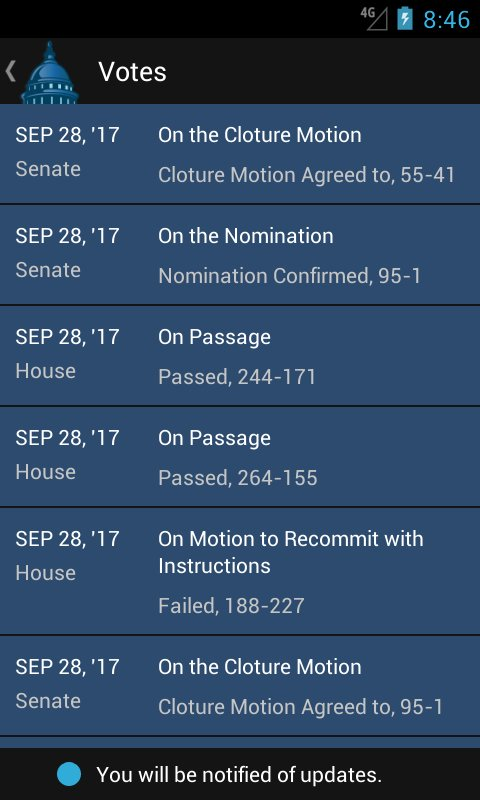
\includegraphics[width=0.5\linewidth]{congress}
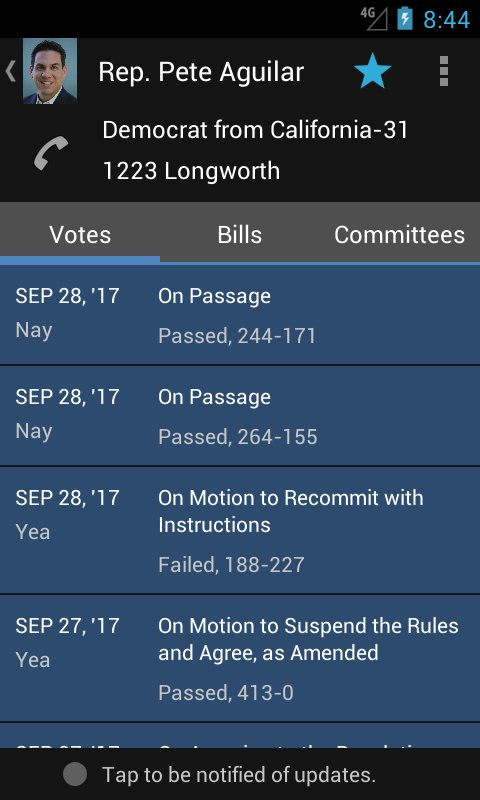
\includegraphics[width=0.5\linewidth]{congress-2}

\section{Zdrojová data}

\subsection{Zdroj}

Zdrojová data PS jsou volně ke stažení na https://www.psp.cz/sqw/hp.sqw?k=1300. Data jsou strukturovaná a pochází z agend PS a Senátu jako např. agenda poslanců, osob, hlasování a tisků. Pro účely této práce nás však budou zajímat pouze podmnožina dat agend z PS, které popíši později. 

\subsection{Formát dat}
Data jsou poskytována v souborech ve formátu UNL, tj.:

\begin{itemize}
	\item Každý řádek v souboru odpovídá jednom řádku v databázi.
	\item Oddělovačem je znak roury (|).
	\item Pokud je sloupec prázdný, je jeho hodnota typu null.
	\item V sloupcích jsou používány tzv. escape sekvence k zápisu speciálních znaků s úvodním znakem \ (backslash) následovaný znakem.
\end{itemize}

Tyto soubory jsou podle typu seskupeny do souborů ve formátu zip, např. poslanci.zip pro data o poslancích a hl-2021ps.zip pro data o hlasováních v 9. volebním období.

\subsection{Aktualizace}

Data obsahují úplný stav, rozdílové aktualizace nejsou poskytovány. To pro nás znamená, že při aktualizaci dat musíme rozdíly mezi zdrojovými daty a daty v databázi najít sami a podle toho aktualizovat databázi. Důležité při tom je to, aby data, která na sobě závisí, byla aktualizována tak, aby byla zaručena jejich konzistence. Tedy pokud při aktualizaci nějakého údaje musíme aktualizovat i všechny údaje, které na tom údaji závisí.

Pokud bude strunktura dat doplňována, budou nové sloupce přidávány na konec. Nové sloupce pro nás nebudou důležitá. Budeme pracovat pouze s daty, které tam jsou v době psaní diplomové práce.

\subsection{Kódování}
Kódování je windows-1250. Ten obsahuje mimo jiné všechny znaky z české abecedy. Na to bude potřeba brát ohled při ukládání dat do databáze, aby se toto kódování zachovalo.

\subsection{Datové typy}
Na stránce je uvedena tabulka obsahující typy dat sloupců v tabulkách a popis jejich významu.

\begin{longtable}{|l|p{9cm}|} \hline
	\multicolumn{2}{|l|}{\textbf{Typy dat sloupců v tabulkách}} \\ \hline
	\textbf{Typ} & \textbf{Popis} \\ \hline
	
	int	& integer \\ \hline
	
	char(X)		& textový řetězec, s blíže neuvedenou délkou
	 \\ \hline
	
	char(N)		& textový řetězec, s konktrétní délkou
	 \\ \hline	
	
	date	& datum, ve formátu DD.MM.YYYY
	 \\ \hline	
	 
 	datetime(year to hour)		& datum a čas, do úrovně hodin, ve formátu YYYY-MM-DD HH
 	
	 \\ \hline
	 
 	datetime(year to second)		& datum a čas, do úrovně vteřin, ve formátu YYYY-MM-DD HH:TT:SS
 	
	 \\ \hline
	 
 	datetime(..., fraction)		& Doplnění formátu o zlomky vteřiny, odděleno tečkou od původního formátu
 	
	 \\ \hline
	 
 	datetime(hour to minute)		& čas, ve formátu HH:MM
	 \\ \hline
	
	\caption{Typy dat sloupců v tabulkách}
	\label{table:data_types}
\end{longtable}

\subsection{Licence}

Data jsou poskytována bezplatně, využití dat je podmíněno uvedením zdroje dat a případně datem zpracování dat. Mobilní aplikace a backend budou implementovány ve dvou různých repozitářích. V každém z nich uvedeno, odkud data pocházela.

\subsection{Tabulky}

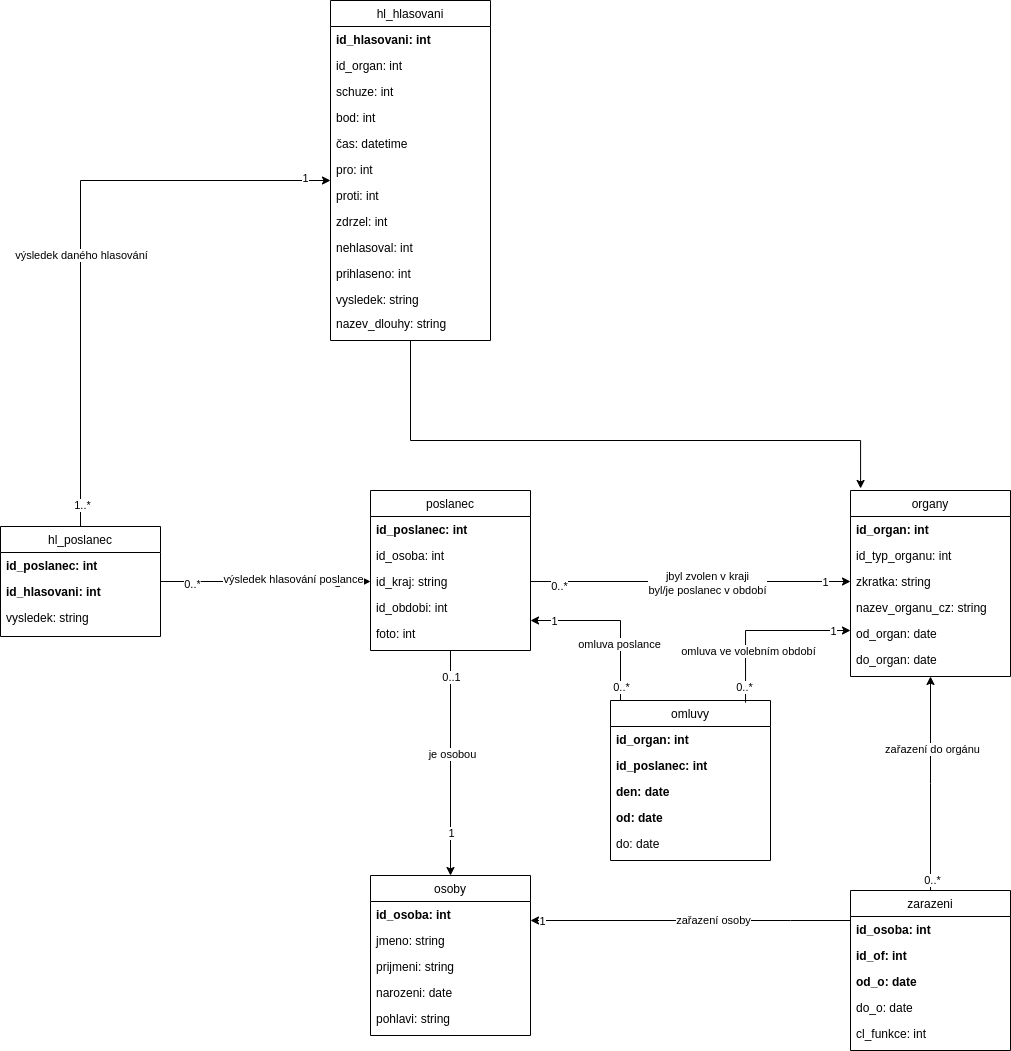
\includegraphics[width=\linewidth]{source_data_diagram}

\subsubsection{typ\textunderscore organu}

Orgány mají svůj typ, tyto typy mají hiearchickou strukturu.

\begin{center}
	\begin{longtable}{|l|l|p{9cm}|}
		\caption{Tabulka typ\textunderscore organu} \label{table:typ_organu} \\
		
		\hline 
		
		\multicolumn{3}{|l|}{\textbf{Tabulka typ\textunderscore organu}} \\
		
		\hline 
		
		\multicolumn{1}{|l|}{\textbf{Sloupec}} & \multicolumn{1}{l|}{\textbf{Typ}} & \multicolumn{1}{l|}{\textbf{Použití a vazby}} \\ 

		\endhead
		
		\hline 
		
		id\textunderscore typ\textunderscore org & int & Identifikátor typu orgánu \\
		
		\hline 
		
		typ\textunderscore id\textunderscore typ\textunderscore org	 org & int & Identifikátor nadřazeného typu orgánu (typ\textunderscore organu:id\textunderscore typ\textunderscore org), pokud je null či nevyplněno, pak nemá nadřazený typ \\
		
		\hline 
		
		nazev\textunderscore typ\textunderscore org\textunderscore cz & char(X) & Název typu orgánu v češtině \\
		
		\hline 
		
		nazev\textunderscore typ\textunderscore org\textunderscore en & char(X) & Název typu orgánu v angličtině \\
		
		\hline 
		
		typ\textunderscore org\textunderscore obecny & int & Obecný typ orgánu, pokud je vyplněný, odpovídá záznamu v typ\textunderscore organu:id\textunderscore typ\textunderscore org. Pomocí tohoto sloupce lze najít např. všechny výbory v různých typech zastupitelských sborů. \\
		
		\hline 
		
		priorita & int & Priorita při výpisu \\
		
		\hline 

	\end{longtable}
\end{center}

\subsubsection{organy}

Některé orgány mají nadřazený orgán a pak je položka organy:organ\textunderscore id\textunderscore organ vyplněna, přičemž pouze v některých případech se tyto vazby využívají.

\begin{center}
	\begin{longtable}{|l|l|p{9cm}|}
		\caption{Tabulka organy} \label{table:organy} \\
		
		\hline 
		
		\multicolumn{3}{|l|}{\textbf{Tabulka organy}} \\
		
		\hline 
		
		\multicolumn{1}{|l|}{\textbf{Sloupec}} & \multicolumn{1}{l|}{\textbf{Typ}} & \multicolumn{1}{l|}{\textbf{Použití a vazby}} \\ 
		
		\endhead
		
		\hline 
		
		id\textunderscore organ & int & Identifikátor orgánu \\
		
		\hline 
		
		organ\textunderscore id\textunderscore organ & int & Identifikátor nadřazeného orgánu, viz organy:id\textunderscore organ \\
		
		\hline 
		
		id\textunderscore typ\textunderscore organu & int & Typ orgánu, viz typ\textunderscore organu:id\textunderscore typ\textunderscore organu \\
		
		\hline 
		
		zkratka & char(X) & Zkratka orgánu, bez diakritiky, v některých připadech se zkratka při zobrazení nahrazuje jiným názvem \\
		
		\hline 
		
		nazev\textunderscore organu\textunderscore cz	 & char(X)	 & Název orgánu v češtině
		 \\
		
		\hline 
		
		nazev\textunderscore organu\textunderscore en	 & char(X)	 & Název orgánu v angličtině
		 \\
		
		\hline 
		
		od\textunderscore organ & date & Ustavení orgánu
		 \\
		
		\hline 
		
		do\textunderscore organ & date & Ukončení orgánu
		 \\
		
		\hline 
		
		priorita & int & Priorita výpisu orgánů
		 \\
		
		\hline 
		
		cl\textunderscore organ\textunderscore base	 & int & Pokud je nastaveno na 1, pak při výpisu členů se nezobrazují záznamy v tabulkce zarazeni kde cl\textunderscore funkce == 0. Toto chování odpovídá tomu, že v některých orgánech nejsou členové a teprve z nich se volí funkcionáři, ale přímo se volí do určité funkce. \\
		
		\hline 
		
	\end{longtable}
\end{center}

\subsubsection{osoby}

Obsahuje jména osob, které jsou zařazeni v orgánech. Vzhledem k tomu, že k jednoznačnému rozlišení osob často není dostatek informací, je možné, že ne všechny záznamy odkazují na jedinečné osoby, tj. některé osoby jsou v tabulce vícekrát.

\begin{center}
	\begin{longtable}{|l|l|p{9cm}|}
		\caption{Tabulka osoby
		} \label{table:osoby} \\
		
		\hline 
		
		\multicolumn{3}{|l|}{\textbf{Tabulka osoby
		}} \\
		
		\hline 
		
		\multicolumn{1}{|l|}{\textbf{Sloupec}} & \multicolumn{1}{l|}{\textbf{Typ}} & \multicolumn{1}{l|}{\textbf{Použití a vazby}} \\ 
		
		\endhead
		
		\hline 
		
		id\textunderscore osoba & int & Identifikátor osoby \\
		
		\hline 
		
		pred & char(X) & Titul pred jmenem \\
	
		\hline 
		
		jmeno & char(X) & Jméno \\
		
		\hline 
		
		prijmeni & char(X) & Příjmení, v některých případech obsahuje i dodatek typu "st.", "ml." \\
		
		\hline 
		
		za & char(X) & Titul za jménem \\
		
		\hline 
		
		narozeni & date & Datum narození, pokud neznámo, pak 1.1.1900. \\
		
		\hline 

		pohlavi & char(X) & Pohlaví, "M" jako muž, ostatní hodnoty žena \\
		
		\hline 
		
		zmena & date & Datum posledni změny \\
		
		\hline 
		
		umrti & date & Datum úmrtí \\
		
		\hline 
		
		
	\end{longtable}
\end{center}

\subsubsection{zarazeni}

Obsahuje data zařazení v orgánu nebo data funkcí osoby v orgánu. Pokud je zarazeni:do\textunderscore o typu null, pak jde o aktuální zařazení.

\begin{center}
	\begin{longtable}{|l|l|p{9cm}|}
		\caption{Tabulka zarazeni} 
		\label{table:zarazeni} \\
		
		\hline 
		
		\multicolumn{3}{|l|}{\textbf{Tabulka zarazeni}} \\
		
		\hline 
		
		\multicolumn{1}{|l|}{\textbf{Sloupec}} & \multicolumn{1}{l|}{\textbf{Typ}} & \multicolumn{1}{l|}{\textbf{Použití a vazby}} \\ 
		
		\endhead
		
		\hline 
		
		id\textunderscore osoba & int & Identifikátor osoby, viz osoba:id\textunderscore osoba \\
		
		\hline 
		
		id\textunderscore of & int & Identifikátor orgánu či funkce: pokud je zároveň nastaveno zarazeni:cl\textunderscore funkce == 0, pak id\textunderscore o odpovídá organy:id\textunderscore organ, pokud cl\textunderscore funkce == 1, pak odpovídá funkce:id\textunderscore funkce.
		 \\
		
		\hline 
		
		cl\textunderscore funkce & int & Status členství nebo funce: pokud je rovno 0, pak jde o členství, pokud 1, pak jde o funkci.
		 \\
		
		\hline 
		
		od\textunderscore o & datetime(year to hour)	 & Zařazení od
		 \\
		
		\hline 
		
		do\textunderscore o & datetime(year to hour)	 & Zařazení do
		 \\
		
		\hline 
		
		od\textunderscore f & date & Mandát od. Nemusí být vyplněno a pokud je vyplněno, pak určuje datum vzniku mandátu a zarazeni:od\textunderscore o obsahuje datum volby.
		 \\
		
		\hline 
		
		do\textunderscore f & date & Mandát do. Nemusí být vyplněno a pokud je vyplněno, určuje datum konce mandátu a zarazeni:do\textunderscore o obsahuje datum ukončení zařazení. \\
		
		\hline 
		
		
	\end{longtable}
\end{center}

\subsubsection{poslanec}

\begin{center}
	\begin{longtable}{|l|l|p{9cm}|}
		\caption{Tabulka poslanec} 
		\label{table:poslanec} \\
		
		\hline 
		
		\multicolumn{3}{|l|}{\textbf{Tabulka poslanec}} \\
		
		\hline 
		
		\multicolumn{1}{|l|}{\textbf{Sloupec}} & \multicolumn{1}{l|}{\textbf{Typ}} & \multicolumn{1}{l|}{\textbf{Použití a vazby}} \\ 
		
		\endhead
		
		\hline 
		
		id\textunderscore poslanec & int & Identifikátor poslance \\
		
		\hline 
		
		id\textunderscore osoba & int & Identifikátor osoby, viz osoba:id\textunderscore osoba \\
		
		\hline 
		
		id\textunderscore kraj & int & Volební kraj, viz organy:id\textunderscore organu \\
		
		\hline 
		
		id\textunderscore kandidatka & int & Volební strana/hnutí, viz org:id\textunderscore organu, pouze odkazuje na stranu/hnutí, za kterou byl zvolen a nemusí mít souvislost s členstvím v poslaneckém klubu. \\
		
		\hline 
		
		id\textunderscore obdobi & int & Volební období, viz organy:id\textunderscore organu \\
		
		\hline 
		
		web & char(X) & URL vlastních stránek poslance \\
		
		\hline 
		
		ulice & char(X) & Adresa regionální kanceláře, ulice. \\
		
		\hline 
		
		obec & char(X) & Adresa regionální kanceláře, obec. \\
		
		\hline 
		
		psc & char(X) & Adresa regionální kanceláře, PSČ. \\
		
		\hline 
		
		email & char(X) & E-mailová adresa poslance, případně obecná posta@psp.cz. \\
		
		\hline 
		
		telefon & char(X) & Adresa regionální kanceláře, telefon. \\
		
		\hline 
		
		fax & char(X) & Adresa regionální kanceláře, fax. \\
		
		\hline 
		
		psp\textunderscore telefon & char(X) & Telefonní číslo do kanceláře v budovách PS. \\
		
		\hline 
		
		facebook & char(X) & URL stránky služby Facebook. \\
		
		\hline 
		
		foto & int & Pokud je rovno 1, pak existuje fotografie poslance. \\
		
		\hline 
		
	\end{longtable}
\end{center}

\subsubsection{hl\textunderscore hlasovani}

\begin{center}
	\begin{longtable}{|l|l|p{9cm}|}
		\caption{Tabulka hl\textunderscore hlasovani} 
		\label{table:hl_hlasovani} \\
		
		\hline 
		
		\multicolumn{3}{|l|}{\textbf{Tabulka hl\textunderscore hlasovani}} \\
		
		\hline 
		
		\multicolumn{1}{|l|}{\textbf{Sloupec}} & \multicolumn{1}{l|}{\textbf{Typ}} & \multicolumn{1}{l|}{\textbf{Použití a vazby}} \\ 
		
		\endhead
		
		\hline 
		
		id\textunderscore hlasovani & int & Identifikátor hlasování \\
		
		\hline 
		
		id\textunderscore organ & int & Identifikátor orgánu, viz organy:id\textunderscore organ	 \\
		
		\hline 
		
		schuze & int & Číslo schůze
		 \\
		
		\hline 
		
		cislo & int & Číslo hlasování
		 \\
		
		\hline 
		
		bod & int & Bod pořadu schůze; je-li menší než 1, pak jde o procedurální hlasování nebo o hlasování k bodům, které v době hlasování neměly přiděleno číslo.
		 \\
		
		\hline 
		
		datum & date & Datum hlasování
		 \\
		
		\hline 
		
		čas & datetime(hour to minute)	 & Čas hlasování
		 \\
		
		\hline 
		
		pro & int & Počet hlasujících pro
		 \\
		
		\hline 
		
		proti & int & Počet hlasujících proti
		 \\
		
		\hline 
		
		zdrzel & int & Počet hlasujících zdržel se, tj. stiskl tlačítko X
		 \\
		
		\hline 
		
		nehlasoval & int & Počet přihlášených, kteří nestiskli žádné tlačítko
		 \\
		
		\hline 
		
		prihlaseno & int & Počet přihlášených poslanců
		 \\
		
		\hline 
		
		kvorum & int & Kvórum, nejmenší počet hlasů k přijetí návrhu
		 \\
		
		\hline 
		
		druh\textunderscore hlasovani & char(X)	 & Druh hlasování: N - normální, R - ruční (nejsou známy hlasování jednotlivých poslanců), E - vinou technické závady nejsou dostupná všechna data k hlasování, např. výsledky hlasování jednotlivých poslanců.
		 \\
		
		\hline 
		
		vysledek & char(X)	 & Výsledek: A - přijato, R - zamítnuto, jinak zmatečné hlasování
		 \\
		
		\hline 
		
		nazev\textunderscore dlouhy & char(X)	 & Dlouhý název bodu hlasování
		 \\
		
		\hline 
		
		nazev\textunderscore kratky & char(X)	 & Krátký název bodu hlasování \\
		
		\hline 
		
	\end{longtable}
\end{center}

\subsubsection{hl\textunderscore poslanec}

Tabulka zaznamenává výsledek hlasování jednotlivého poslance.

\begin{center}
	\begin{longtable}{|l|l|p{9cm}|}
		\caption{Tabulka hl\textunderscore poslanec} 
		\label{table:hl_hlasovani} \\
		
		\hline 
		
		\multicolumn{3}{|l|}{\textbf{Tabulka hl\textunderscore poslanec}} \\
		
		\hline 
		
		\multicolumn{1}{|l|}{\textbf{Sloupec}} & \multicolumn{1}{l|}{\textbf{Typ}} & \multicolumn{1}{l|}{\textbf{Použití a vazby}} \\ 
		
		\endhead
		
		\hline 
		
		id\textunderscore poslanec & int & Identifikátor poslance, viz poslanec:id\textunderscore poslanec
		 \\
		
		\hline 
		
		id\textunderscore hlasovani & int & Identifikátor hlasování, viz hl\textunderscore hlasovani:id\textunderscore hlasovani
		\\
		
		\hline 
		
		vysledek & char(X) & Hlasování jednotlivého poslance. 'A' - ano, 'B' nebo 'N' - ne, 'C' - zdržel se (stiskl tlačítko X), 'F' - nehlasoval (byl přihlášen, ale nestiskl žádné tlačítko), '@' - nepřihlášen, 'M' - omluven, 'W' - hlasování před složením slibu poslance, 'K' - zdržel se/nehlasoval. Viz úvodní vysvětlení zpracování výsledků hlasování.
		\\
		
		\hline 
		
	\end{longtable}
\end{center}

\subsubsection{omluvy}

Tabulka zaznamenává časové ohraničení omluv poslanců z jednání Poslanecké sněmovny.

\begin{center}
	\begin{longtable}{|l|l|p{9cm}|}
		\caption{Tabulka omluvy} 
		\label{table:omluvy} \\
		
		\hline 
		
		\multicolumn{3}{|l|}{\textbf{Tabulka omluvy}} \\
		
		\hline 
		
		\multicolumn{1}{|l|}{\textbf{Sloupec}} & \multicolumn{1}{l|}{\textbf{Typ}} & \multicolumn{1}{l|}{\textbf{Použití a vazby}} \\ 
		
		\endhead
		
		\hline 
		
		id\textunderscore organ & int & Identifikátor volebního období, viz organy:id\textunderscore organ
			\\
		
		\hline 
		
		id\textunderscore poslanec & int & Identifikátor poslance, viz poslanec:id\textunderscore poslanec
			\\
		
		\hline 
		
		
		den & date & Datum omluvy
			\\
		
		\hline 
		
		
		od & datetime(hour to minute)	 & Čas začátku omluvy, pokud je null, pak i omluvy:do je null a jedná se o omluvu na celý jednací den.
			\\
		
		\hline 
		
		
		do & datetime(hour to minute)	 & Čas konce omluvy, pokud je null, pak i omluvy:od je null a jedná se o omluvu na celý jednací den.	\\
		
		\hline 
		
	\end{longtable}
\end{center}







\chapter{Analýza zdrojových dat}
\label{ch:analysis_data}
\setcounter{page}{1}

V této kapitole budou analyzována zdrojová data, z kterých bude čerpat backend.

\section{Zdrojové soubory}

Zdrojová data se nachází v souborech ve formátu zip, které jsou volně ke stažení na \href{https://www.psp.cz/sqw/hp.sqw?k=1300}{\color{blue}stránkách} PSP. Pro tuto práci budou důležité následující soubory, které obsahují datové soubory potřebné pro splnění zadání a funkčních a nefunkčních požadavků:

\begin{itemize}
	\item \textbf{poslanci.zip} - Eviduje osoby, jejich zařazení do orgánů a jejich funkce v orgánech a orgány jako takové. Obsahuje datové soubory potřebné 
	\item \textbf{hl-XXXXps.zip} - Eviduje hlasování v PS.
\end{itemize}

\noindent Zbytek práce se bude zabývat daty v datových souborech v těchto dvou zdrojových souborech.

\section{Formát dat}
Data v datových souborech jsou poskytována ve formátu UNL, tj.:

\begin{itemize}
	\item Každý řádek v souboru odpovídá jednom řádku v databázi.
	\item Oddělovačem je znak roury (|).
	\item Pokud je sloupec prázdný, je jeho hodnota typu null.
	\item V sloupcích jsou používány tzv. escape sekvence k zápisu speciálních znaků s úvodním znakem \ (backslash) následovaný znakem.
\end{itemize}

\noindent Další informace o datech:

\begin{itemize}
	\item Kódování dat je windows-1250
	\item Pokud bude strunktura dat doplňována, budou nové sloupce přidávány na konec.
\end{itemize}

\noindent Kódování windows-1250 obsahuje mimo jiné všechny znaky z české abecedy. Je tedy třeba dbát na správně nastavené kódování při parsování nebo ukládání do databáze, aby datům vráceným mobilní aplikaci nechyběly např. háčky a čárky. Zároveň při parsování UNL souborů je potřeba brát ohled na přidávání nových sloupců nakonec.

\section{Aktualizace}

\href{https://www.psp.cz/sqw/hp.sqw?k=1300}{\color{blue}Web} uvádí, že data obsahují úplný stav a že rozdílové aktualizace nejsou poskytovány. To je pro použití neideální, jelikož při aktualizaci dat je potřeba stáhnout všechna data a následně buď zpracovat všechna data znovu nebo naimplementovat vlastní logiku pro zjištění rozdílového stavu a aktualizovat data pouze na základě tohoto rozdílového stavu. 

\section{Datové typy}
Na \href{https://www.psp.cz/sqw/hp.sqw?k=1300}{\color{blue}stránce} jsou poskytovány informace o datových typech sloupců. Zde je výčet pouze těch datových typů, které jsou nutné pro pochopení dat používaných v rámci této práce.

\begin{longtable}{|l|p{9cm}|} \hline
	\multicolumn{2}{|l|}{\textbf{Typy dat sloupců v tabulkách}} \\ \hline
	\textbf{Typ} & \textbf{Popis} \\ \hline
	
	int	& integer \\ \hline
	
	char(X)		& textový řetězec, s blíže neuvedenou délkou
	\\ \hline

	date	& datum, ve formátu DD.MM.YYYY
	\\ \hline	
	
	datetime(year to hour)		& datum a čas, do úrovně hodin, ve formátu YYYY-MM-DD HH
	
	\\ \hline
	
	datetime(hour to minute)		& čas, ve formátu HH:MM
	\\ \hline
	
	\caption{Datové typy dat}
	\label{table:data_types}
\end{longtable}

\section{Licence}

Data jsou poskytována bezplatně, využití dat je podmíněno uvedením zdroje dat a případně datem zpracování dat. V mobilní aplikaci a v repozitářích mobilní aplikace a backendu bude uveden zdroj dat. 

\section{Datové soubory}

Zde je výčet použitých datových souborů a stručná analýza. Detailnější analýza bude v následující sekci. Ze zdrojového souboru \lstinline|poslanci.zip| budou používány následující datové soubory (\cite{zip-members}:)

\begin{itemize}
	\item \textbf{organy} - Reprezentuje orgány ve státní správě. Zahrnuje parlamenty všech volebních období a poslanecké kluby. Tabulka bude využita pro nalezení všech poslaneckých klub;.
	\item \textbf{poslanec} - Reprezentuje poslance v různých volebních obdobích.
	\item \textbf{osoby} - Reprezentuje osobu. Obsahuje osobní údaje jako jméno a příjmení a datum narození. Poslanec je osobou, a tudíž lze o poslanci prostřednictvím téhle tabulky zjistit jeho osobní údaje.
	\item \textbf{zarazeni} - Obsahuje zařazení osoby osoby do nějakého orgánu. Tabulka bude využita pro zjištění členů poslaneckého klubu.
\end{itemize}

\noindent Ze zdrojových souborů \lstinline|hl-XXXX.zip|, kde XXXX je volební rok, budou používány následující datové soubory (\cite{zip-votes}:)

\begin{itemize}
	\item \textbf{hl\_hlasovani} - Reprezentuje hlasování o návrhu zákona. Zahrnuje většinu informací o hlasování, které budou potřeba.
	\item \textbf{hl\_poslanec} - Reprezentuje výsledek hlasování poslance o návrhu zákona, tedy jak hlasoval který poslanec o kterém návrhu zákona.
	\item \textbf{omluvy} - Repreznetuje časově ohraničené omluvy z jednání a hlasování v poslanecké sněmovně. Bude použito pro zjištění počtu omluvených. 
\end{itemize}

\section{Tabulky}

Na (\ref{fig:class-diagram}) lze vidět diagram zdrojových dat, s kterými bude dále v práci pracováno. Obsahuje typy dat, jejich atributy, datové typy atributů a vazby mezi typy. Atributy identifikující daný typ jsou zvýrazněny tučným písmem. Následovat bude výčet použitých tabulek s popisem atributů. Pro stručnost budou u tabulek uvedeny pouze atributy, které jsou v rámci práce používány. Poznatky v textu jsou převážně z \textbf{analýzy obsahu datových souborů} a nejsou na stránkách PS nijak zdokumentovány.

\subsection*{organy}
Tabulka \textbf{organy} (\ref{table:organy}) bude použita pro nalezení poslaneckých klubů v určitém volebním období. Všechny poslanecké kluby mají hodnotu atributu \textbf{id\_typ\_organu} rovnou 1. Poslanecké kluby v daném volebním období lze nalézt kontrolou, zda hodnoty atributů \textbf{od\_organ} a \textbf{do\_organ} spadají mezi hodnotami stejných atributů PS. PS je totiž také orgánem a lze ji najít prostřednictvím hodnoty atributu \textbf{id\_organ}. První PS má identifikátor 165. PS v každém následujícím volebním období má hodnotu identifikátoru o jednu větší než PS v předchozím volebním období. Tedy např. PS ve volebním období 2017 až 2021 má identifikátor 172. Dále pokud hodnota atributu \textbf{do\_organ} je rovna \lstinline|null|, pak jde o aktuální orgán.

\begin{center}
	\begin{longtable}{|l|l|p{9cm}|}
		\caption{Tabulka organy} \label{table:organy} \\
		
		\hline 
		
		\multicolumn{3}{|l|}{\textbf{Tabulka organy}} \\
		
		\hline 
		
		\multicolumn{1}{|l|}{\textbf{Sloupec}} & \multicolumn{1}{l|}{\textbf{Typ}} & \multicolumn{1}{l|}{\textbf{Použití a vazby}} \\ 
		
		\endhead
		
		\hline 
		
		id\textunderscore organ & int & Identifikátor orgánu \\
		
		\hline 
		
		id\textunderscore typ\textunderscore organu & int & Identifikátor typu orgánu \\
		
		\hline 
		
		zkratka & char(X) & Zkratka orgánu \\
		
		\hline 
		
		nazev\textunderscore organu\textunderscore cz	 & char(X)	 & Název orgánu v češtině
		\\
		
		\hline 
		
		od\textunderscore organ & date & Datum ustavení orgánu
		\\
		
		\hline 
		
		do\textunderscore organ & date & Datum ukončení orgánu
		\\
		
		\hline 
		
	\end{longtable}
\end{center}

\subsection*{osoby}

Tabulka \textbf{osoby} (\ref{table:osoby}) bude použita pro získání osobních údajů o poslancích. Tabulka však nezahrnuje pouze poslance, ale i další osoby senátu. Pro zjištění, kterého poslance reprezentuje daná osoba, je potřeba použít tabulku \textbf{zarazeni}. Zde je zajímavé datum narození, které je 1. 1. 1900, pokud je neznámo. Zobrazovat toto datum v mobilní aplikaci by nebylo ideální. V kapitole o návrhu REST API bude popsána transformace tohoto data na jinou hodnotu.

\begin{center}
	\begin{longtable}{|l|l|p{9cm}|}
		\caption{Tabulka osoby
		} \label{table:osoby} \\
		
		\hline 
		
		\multicolumn{3}{|l|}{\textbf{Tabulka osoby
		}} \\
		
		\hline 
		
		\multicolumn{1}{|l|}{\textbf{Sloupec}} & \multicolumn{1}{l|}{\textbf{Typ}} & \multicolumn{1}{l|}{\textbf{Použití a vazby}} \\ 
		
		\endhead
		
		\hline 
		
		id\textunderscore osoba & int & Identifikátor osoby \\
		
		\hline 
		
		jmeno & char(X) & Jméno \\
		
		\hline 
		
		prijmeni & char(X) & Příjmení \\
		
		\hline 
		
		narozeni & date & Datum narození, pokud neznámo, pak 1.1.1900. \\
		
		\hline 
		
		pohlavi & char(X) & Pohlaví, "M" jako muž, ostatní hodnoty žena \\
		
		\hline 
		
		
	\end{longtable}
\end{center}

\subsection*{zarazeni}

Tabulka zařazení bude použita ke zjištění příslušnosti poslance do poslaneckého klubu. Zde je potřeba dát pozor na to, že atribut \textbf{id\_of} může reprezentovat buď tabulku \textbf{organ} (tu používáme) nebo tabulku \textbf{funkce} (tu nepoužíváme, a tudíž tu není uvedena) podle toho, zda je hodnota atributu \textbf{cl\_funkce} rovna 0 nebo 1. Tabulka \textbf{funkce} reprezentuje konkrétní funkci v daném orgánu. Pro účely této práce tato informace není potřeba, a proto tu tabulka \textbf{funkce} není uvedena. Je však potřeba zjistit příslušnost poslance do poslaneckého klubu, kterou lze zjistit kombinací tabulky \textbf{zarazeni} a \textbf{organy}. Důsledkem popsaného je to, že nás budou zajímat pouze zařazení s hodnotou atributu \textbf{cl\_funkce} rovnou 0. Tím pádem identifikátor \textbf{id\_of} bude vždy referovat k tabulce \textbf{organy}. Tabulka \textbf{organy} obsahuje poslanecké kluby, což je přesně to, co potřebujeme. Dále pokud hodnota atributu \textbf{do\_o} je rovna \lstinline|null|, pak jde o aktuální zařazení.

\begin{center}
	\begin{longtable}{|l|l|p{9cm}|}
		\caption{Tabulka zarazeni} 
		\label{table:zarazeni} \\
		
		\hline 
		
		\multicolumn{3}{|l|}{\textbf{Tabulka zarazeni}} \\
		
		\hline 
		
		\multicolumn{1}{|l|}{\textbf{Sloupec}} & \multicolumn{1}{l|}{\textbf{Typ}} & \multicolumn{1}{l|}{\textbf{Použití a vazby}} \\ 
		
		\endhead
		
		\hline 
		
		id\textunderscore osoba & int & Identifikátor osoby, viz osoba:id\textunderscore osoba \\
		
		\hline 
		
		id\textunderscore of & int & Identifikátor orgánu či funkce: pokud je zároveň nastaveno zarazeni:cl\textunderscore funkce == 0, pak id\textunderscore o odpovídá organy:id\textunderscore organ, pokud cl\textunderscore funkce == 1, pak odpovídá funkce:id\textunderscore funkce.
		\\
		
		\hline 
		
		cl\textunderscore funkce & int & Status členství nebo funkce: pokud je rovno 0, pak jde o členství, pokud 1, pak jde o funkci.
		\\
		
		\hline 
		
		od\textunderscore o & datetime(year to hour)	 & Zařazení od
		\\
		
		\hline 
		
		do\textunderscore o & datetime(year to hour)	 & Zařazení do
		\\
		
		\hline 
		
	\end{longtable}
\end{center}

\subsection*{poslanec}

Tabulka \textbf{poslanec} (\ref{table:poslanec}) slouží pro získání informací o všech poslancích. Pokud je někdo poslancem ve více volebních obdobích, pak bude v této tabulce mít více záznamů. Tedy dva poslanci mohou reprezentovat tutéž osobu, pokud jsou z různých volebních období. Dále pomocí atributu \textbf{id\_osoba} lze tabulku zjistit osobní údaje o poslanci. Dále pomocí atributu \textbf{id\_kraj} lze získat název volebního kraje. A pomocí atributu \textbf{id\_obdobi} lze zjisti volební období, do kterého přísluší. Hodnota atributu \textbf{id\_obdobi} totiž odpovídá identifikátoru některé z PS. Např. pokud poslanec patří do PS v prvním volebním období (orgán mající identifikátor 165), pak je hodnota atributu \textbf{id\_obdobi} rovna 165. Dále někteří poslanci mají profilové foto. Po analýze fotek poslanců na oficiálním portálu PS byl zjištěn následující vzor pro URL fotky poslance: \lstinline|https://www.psp.cz/eknih/cdrom/XXXXps/eknih/XXXXps/poslanci/iYYY.jpg|, kde \lstinline|XXXX| je identifikátor osoby (pozor, ne identikátor poslance) a \lstinline|YYY| je identifikátor PS (např. 165). Příklad: pokud bychom chtěli najít URL s fotkou poslance s identifikátorem 1659, zjistíme hodnoty atributů \textbf{id\_kraj} a \textbf{id\_obdobi}, a na základě nich vygenerujeme URL fotky.

\begin{center}
	\begin{longtable}{|l|l|p{9cm}|}
		\caption{Tabulka poslanec} 
		\label{table:poslanec} \\
		
		\hline 
		
		\multicolumn{3}{|l|}{\textbf{Tabulka poslanec}} \\
		
		\hline 
		
		\multicolumn{1}{|l|}{\textbf{Sloupec}} & \multicolumn{1}{l|}{\textbf{Typ}} & \multicolumn{1}{l|}{\textbf{Použití a vazby}} \\ 
		
		\endhead
		
		\hline 
		
		id\textunderscore poslanec & int & Identifikátor poslance \\
		
		\hline 
		
		id\textunderscore osoba & int & Identifikátor osoby, viz osoba:id\textunderscore osoba \\
		
		\hline 
		
		id\textunderscore kraj & int & Volební kraj, viz organy:id\textunderscore organu \\
		
		\hline 
		
		id\textunderscore obdobi & int & Volební období, viz organy:id\textunderscore organu \\
		
		\hline 
		
		foto & int & Pokud je rovno 1, pak existuje fotografie poslance. \\
		
		\hline 
		
	\end{longtable}
\end{center}

\subsection*{hl\textunderscore hlasovani}

Tabulka \textbf{hl\_hlasovani} obsahuje většinu potřebných informací o hlasováních o daném návrhu zákona. Čislo schůze a číslo hlasování budou použity pro sestavení URL pro stenoprotokol daného hlasování. Podle webu se od účinnosti novely jednacího řádu 90/1995 Sb. nerozlišuje zdržel se a nehlasoval, tj. příslušné počty se sčítají. Z toho plyne, že by mobilní aplikaci měla u hlasováních uskutečněných před účinností této novely mít kolonku pro počet poslanců, kterí nehlasovali. 
A u hlasováních uskutečněných po účinnosti této novely by tam daná kolonka již být neměla.

\begin{center}
	\begin{longtable}{|l|l|p{9cm}|}
		\caption{Tabulka hl\textunderscore hlasovani} 
		\label{table:hl_hlasovani} \\
		
		\hline 
		
		\multicolumn{3}{|l|}{\textbf{Tabulka hl\textunderscore hlasovani}} \\
		
		\hline 
		
		\multicolumn{1}{|l|}{\textbf{Sloupec}} & \multicolumn{1}{l|}{\textbf{Typ}} & \multicolumn{1}{l|}{\textbf{Použití a vazby}} \\ 
		
		\endhead
		
		\hline 
		
		id\textunderscore hlasovani & int & Identifikátor hlasování \\
		
		\hline 
		
		schuze & int & Číslo schůze
		\\
		
		\hline 
		
		cislo & int & Číslo hlasování
		\\
		
		\hline 
		
		datum & date & Datum hlasování
		\\
		
		\hline 
		
		čas & datetime(hour to minute)	 & Čas hlasování
		\\
		
		\hline 
		
		pro & int & Počet hlasujících pro
		\\
		
		\hline 
		
		proti & int & Počet hlasujících proti
		\\
		
		\hline 
		
		zdrzel & int & Počet hlasujících zdržel se, tj. stiskl tlačítko X
		\\
		
		\hline 
		
		nehlasoval & int & Počet přihlášených, kteří nestiskli žádné tlačítko
		\\
		
		\hline 
		
		prihlaseno & int & Počet přihlášených poslanců
		\\
		
		\hline 
		
		vysledek & char(X)	 & Výsledek: A - přijato, R - zamítnuto, jinak zmatečné hlasování
		\\
		
		\hline 
		
		nazev\textunderscore dlouhy & char(X)	 & Dlouhý název bodu hlasování
		\\
		
		\hline 
		
	\end{longtable}
\end{center}

\subsection*{hl\textunderscore poslanec}

Tabulka \textbf{hl\_poslanec} obsahue informace o tom, jak hlasoval který poslanec v rámci kterého hlasování. Výsledky 'B' a 'N' jsou interpretovány stejně, oba znamenají hlasování proti. Výsledek 'Fb se používalo před rokem 1995. Po roce 1995 má vždy hodnotu 0. Výsledek 'W' je velmi ojedinělý a v případě, že nastane, sečte se do počtu nepřihlášených. U výsledku 'K' se mi nepodařilo zjistit, co přesně znamená zdržel se/nehlasoval. Ve zdrojových datech se vysktuje spíš méně, ale častěji než výsledek 'W'. Na webu PS je tento výsledek u jednoho hlasování v roce 2013 interpretován jako nehlasoval. Z toho lze usoudit pouze to, že 'K' může znamenat nehlasoval. Není však z toho jasné, kdy může znamenat zdržel se. Na výsledek hlasování má vliv pouze počet pro a proti, a tudíž bylo rozhodnuto, že tento výsledek bude mobilní aplikaci ignorován. 

\begin{center}
	\begin{longtable}{|l|l|p{9cm}|}
		\caption{Tabulka hl\textunderscore poslanec} 
		\label{table:hl_poslanec} \\
		
		\hline 
		
		\multicolumn{3}{|l|}{\textbf{Tabulka hl\textunderscore poslanec}} \\
		
		\hline 
		
		\multicolumn{1}{|l|}{\textbf{Sloupec}} & \multicolumn{1}{l|}{\textbf{Typ}} & \multicolumn{1}{l|}{\textbf{Použití a vazby}} \\ 
		
		\endhead
		
		\hline 
		
		id\textunderscore poslanec & int & Identifikátor poslance, viz poslanec:id\textunderscore poslanec
		\\
		
		\hline 
		
		id\textunderscore hlasovani & int & Identifikátor hlasování, viz hl\textunderscore hlasovani:id\textunderscore hlasovani
		\\
		
		\hline 
		
		vysledek & char(X) & Hlasování jednotlivého poslance. 'A' - ano, 'B' nebo 'N' - ne, 'C' - zdržel se, 'F' - nehlasoval, '@' - nepřihlášen, 'M' - omluven, 'W' - hlasování před složením slibu poslance, 'K' - zdržel se/nehlasoval.
		\\
		
		\hline 
		
	\end{longtable}
\end{center}

\subsection*{omluvy}

Tabulka \textbf{omluvy} (\ref{table:omluvy}) zaznamenává časové ohraničení omluv poslanců z jednání Poslanecké sněmovny. Slouží pouze po spočtení počtu omluvených poslanců během hlasování. Podáváme-li se na statistiky o hlasování poskytnuté tabulkou \textbf{hl\_hlasovani}, uvidíme, že poskytuje počet hlasování pro, proti, a počet zdržených, ale již ne počet nepřihlášených a omluvených. Počet omluvených byl přidán až po 1995, kdy pouze nahradil počet poslanců, kteří nehlasovali. Počet nehlasujících poslanců tedy nepomůže k odvození počtu nepřihlášených a omluvených. Jediná další informace v tabulce \textbf{hl\_hlasovani} je tedy počet přihlášených. Intuitivně by člověk čekal, že doplněk pro počet přihlášených je počet nepřihlášených, ale není tomu tak. Když jsem od počtu poslanců (200) odečetl počet přihlášených, nikdy to nevycházelo s počty nepřihlášených na webu, ať už jsem to zkoušel s jakýmkoliv hlasování. Z toho důvodu je počet omluvených počítáno z tabulky \textbf{omluvy}, kde na základě atributů \textbf{den}, \textbf{od} a \textbf{do} zjistíme, zda datum a čas omluvy poslance spadá do data a času daného hlasování.

Podle popisu tabulky na webu data slouží pro nahrazení výsledku typu '@', tj. pokud výsledek hlasování jednotlivého poslance je nepřihlášen. Pokud čas hlasování spadá do časového intervalu omluvy, pak se za výsledek považuje 'M', tj. omluven.

\begin{center}
	\begin{longtable}{|l|l|p{9cm}|}
		\caption{Tabulka omluvy} 
		\label{table:omluvy} \\
		
		\hline 
		
		\multicolumn{3}{|l|}{\textbf{Tabulka omluvy}} \\
		
		\hline 
		
		\multicolumn{1}{|l|}{\textbf{Sloupec}} & \multicolumn{1}{l|}{\textbf{Typ}} & \multicolumn{1}{l|}{\textbf{Použití a vazby}} \\ 
		
		\endhead
		
		\hline 
		
		id\textunderscore organ & int & Identifikátor volebního období, viz organy:id\textunderscore organ
		\\
		
		\hline 
		
		id\textunderscore poslanec & int & Identifikátor poslance, viz poslanec:id\textunderscore poslanec
		\\
		
		\hline 
		
		
		den & date & Datum omluvy
		\\
		
		\hline 
		
		
		od & datetime(hour to minute)	 & Čas začátku omluvy, pokud je null, pak i omluvy:do je null a jedná se o omluvu na celý jednací den.
		\\
		
		\hline 
		
		
		do & datetime(hour to minute)	 & Čas konce omluvy, pokud je null, pak i omluvy:od je null a jedná se o omluvu na celý jednací den.	\\
		
		\hline 
		
	\end{longtable}
\end{center}
\chapter{Technologie}

\setcounter{page}{1}

\section{Programovací jazyky}

\subsection{Java}

Java je objektově-orientovaný, staticky typovaný programovací jazyk  jazyk, který byl navržen tak, aby byl portabilní a bezpečný. Portabilní a bezpečný je díky tomu, že běží na virtuálním stroji, který interpretuje mezikód, do kterého je kód Javy kompilován. Ten funguje na mnoha platformách včetně Windows, Mac OS a Linux. Java používá automatickou správu paměti, díky které není potřeba manuálně uvolňovat naalokované paměti, které by jinak způsobily memory leak. Java se používá mimo jiné pro enterprise aplikace a je hlavním jazykem pro vývoj Androidích aplikací. Od roku 2017 začal Google však podporovat Kotlin jako hlavní programoací jazyk pro vývoj v Androidu. 

\subsection{Kotlin}
Kotlin je staticky-typovaný jazyk, který klade důraz na bezpečnost, čitelnost a stručnost kódu. Narozdíl od Javy podporuje např. null safety, extension funkce a coroutines. Je s Javou plně interoperabilní, tj. dokážeme v Kotlinu volat metody a používat knihovny napsaně v Javě. Kotlin byl Googlem uznán jako hlavní jazyk pro vývoj aplikací pro Android. 

\subsection{Závěr}
Pro vývoj mobilní aplikace pro Android jsem se rozhodl používat programovací jazyk Kotlin. Prvním důvodem je to, že Kotlin je od roku 2017 Googlem uznán jako hlavní programovací jazyk pro Android. To mělo podle mě za následky, že většina dokumentací, tutoriálů a diskuzí ohledně vývoji androidích aplikací budou používat kód v Kotlinu. Druhým důvodem je to, že kód psaný v Kotlinu je bezpečnější, čitelnější a stručnější. Oba důvody přispívají k snadnější implementaci.

Pro vývoj backendu jsem se rozhodl pro Javu. Důvod pro toto rozhodnutí souvisí s výběrem technologie Spring Boot, kterou jsem použil pro implementaci REST API. Ten popíši v následující podkapitole.

\section{Backend}

\subsection{Spring Framework}
Spring Framework je framework pro vývoj enterprise aplikací. Je založený na principu inversion of control (dále jen IoC), který umožňuje oddělit odpověděnosti a decouplovat komponenty v aplikaci. Díky tomu je aplikace udržitelnější, protože změna jedné komponenty nerozbije ostatní komponenty, pokud jsou rozhraní, přes které komponenty mezi sebou komunikují, nezměněné. Také se aplikace díky tomu lépe testují, protože pro závislosti mezi komponentami lze používat mocky. Zároveň Spring poskytuje různé fíčury pro snazší přístup k datům, implementaci bezpečnosti a webových služeb. Zdroje: https://docs.spring.io/spring-framework/docs/current/reference/html/, https://spring.io/)

\subsection{Spring Boot}
Spring Boot je framework pro vývoj enterprise aplikací. Je postaven nad Spring Frameworkem a klade důraz na konvence nad konfigurací. To znamená, že ve Spring Bootu má mnoho konfigurací defaultní hodnoty, a není třeba je tedy konfigurovat. Konvence byly vybrány podle toho, jak vývojáři většinou používají klasický Spring. Díky tomu je vývoj ve Spring Bootu o dost rychlejší. Dále umožňuje automaticky nakonfigurovat a najít závislosti mezi komponentammi, a tím je objekty mezi sebou pospojovat. Vyžaduje minimální setup a snadnou integraci s technologiemi. 

Zdroje: https://docs.spring.io/spring-framework/docs/current/reference/html/, https://spring.io/)

\subsection{Závěr}

Pro vývoj backendu jsem zvolil technologii Spring Boot. Díky důrazu na konvenci byla implementace mnohem snazší.

Hlavním programovacím jazykem pro vývoj ve Spring Bootu je Java. Nicméně existuje integrace s Kotlinem, která umožňuje psát ve Spring Bootu pomocí Kotlinu. Výhody Kotlinu oproti Javě jsme si popsali v sekci o programovacích jazycích. Nicméně výhoda Javy v kontextu Spring Bootu je ta, že Java ma větší podporu v komunitě, co se týče Spring Bootu. Dokumentace a tutoriály pro Spring Boot jsou psané v Javě (v málo případech pro Kotlin), diskuze jsou také v Javě a když při vývoji narazím na chybu, je snazší nalézt řešení, pokud se chyba týče Javy než Kotlinu. vývoj aplikace ve Spring Bootu v Javě mi tedy připadal rychlejší než v Kotlinu, přestože Kotlin jako programovací jazyk je pro mě lepší.

\section{Databáze}

\subsection{MySQL}
MySQL je systém pro správu relačních databází. Je známá pro svoji spolehlivost, jednoduché použití a výkon. Pro dotazování nad daty používá jazyk SQL. Je multiplatformní, dokáže běžet na operačních systémech Windows, Linux a Mac OS. Je poskytován pod licencí GNU/GPL. Umožňuje transakční zpracování dat. Zdroje: https://www.mysql.com/

\subsection{Závěr}
Pro účely této práce je jediným požadavkem po databázi persistení uložení dat. Databáze MySQL tento požadavek splňuje a mám s ním zkušenosti, a tudíž další varianty již neanalyzuji.

\section{DI framework}


\chapter{Návrh}

\section{Uživatelské rozhraní}

\section{REST API}

\section{Datová struktura}


\chapter{Implementace}
\setcounter{page}{1}

Tato kapitola se zabývá popisem použitých technologií při vývoji mobilní aplikace a backendu,
a způsoby jejich aplikace.

\section{Mobilní aplikace}

\subsection{Programocí jazyk}

\subsubsection *{Kotlin}
Pro mobilní aplikaci byl použit programovací jayzk Kotlin (zdroj: https://kotlinlang.org/), který je od roku 2017 preferovaným jazykem pro Android (zdroj: https://techcrunch.com/2019/05/07/kotlin-is-now-googles-preferred-language-for-android-app-development/). Původním programovacím jayzkem pro Android byla Java (zdroj: https://www.oracle.com/java/), Kotlin má však oproti němu několik výhod. Kód psaný v Kotlin je:

\begin{itemize}
    \item \textbf{stručný} - Kotlin umožňuje vytvořit 
    singleton pomocí klíčového slova \lstinline{object}. (zdroj: https://kotlinlang.org/docs/object-declarations.html)
    \item \textbf{bezpečný} - Kotlin rozlišuje null a non-null datové typy. Non-null typy lze dereferencovat vždy, null typy pouze po kontrole výskytu hodnoty null. To je vynuceno typovým systémem Kotlinu. Díky tomu není možné zkompilovat kód, v kterém by se dereferencovala hodnota null, kvůli čemuž by aplikace spadla. (zdroj: https://kotlinlang.org/docs/null-safety.html)
    \item \textbf{expresivní} - Kotlin byl navržen s důrazem na výstižnost kódu, což přispívá k čitelnosti kódu
\end{itemize}

\subsubsection *{Kotlin Coroutine}
Kotin Coroutine je návrhový vzor, který umožňuje psaní asynchronního kódu, který je intuitivní a efektivní. Asynchronní kód je takový kód, který neblokuje aktuální vlákno. Takový kód se hodí např. pro síťové nebo databázové operace. Z uživatelského hlediska je zajištění asynchronicity dlouhotrvajícího kódu důležité především proto, aby se nezablokovalo vlákno, které má na starosti vykreslování obrazovky a obsluhu událostí jako kliknutí na tlačítko. U Androidí aplikace se tomuto vláknu říká hlavní vlákno a při jejím delším zablokování může uživatelovi naskočit chyba, že aplikace nereaguje na události.

Asynchronní kód lze implementovat i pommocí vláken. Coroutines však mají oproti vláknům následující výhody:

\begin{itemize}
	\item Zabírají méně paměti a lze jich spustit více najednou než vláken. Při vytvoření příliš velkého množství vláken se může zahltit procesor. Vytvořením coroutine se však nevytvoří nové vlákno, ale běží v rámci něj. To znamená, že lze vytvořit tisíce coroutines v rámci jednoho vlákna, které by běžely všechny plynule a asynchronně.
	\item Mají lepší ochranu proti úniku paměti.
	Coroutina může volat další coroutiny. Rodičovská vždy před jejím ukončením počká na to, až dojedou všechny potomkové coroutiny, díky čemuž se vyhneme úniku dat.
\end{itemize}

\subsubsection* {Kotlin Flows}

\subsection{Android SDK}
Android SDK open-source platforma, která poskytuje kolekce nástrojů a API pro vývoj a testování mobilních aplikací, včetně vývojového prostředí, knihoven, emulátoru a testovacích nástrojů.

\subsection {Android Studio \& Android Emulator}

\subsubsection *{Android Studio}

Mobilní aplikace byla vyvíjena ve vývojovém prostředí (dále jen IDE) Android Studio. Byl vyvinut Googlem v roce 2013 a je to preferované IDE pro vývoj Androidích aplikací. Poskytuje napovídání při psaní kódu, automatické dokončování kódu, kontrolu chyb a možnost snadného refaktoringu. Dále poskytuje nástroje pro testování a debugování mobilní aplikace. Obsahuje podporu pro často používané frameworky jako Gradle pro automatické sestavování programu a Android SDK pro sadu vývojových nástrojů.

zdroj: https://developer.android.com/studio

\subsubsection *{Android Emulator}

Pro manuální testování mobilní aplikace byl použit Android Emulator, který simuluje fyzické mobilní zařízení. Jeho výhodou je možnost spouštění, testování a debugování různých modelů zařízení bez jejich vlastnictví. Další výhodou je, že emulátor je vestavěný do IDE vedle zdrojového kódu. Nevýhodou je jeho paměťová a výpočetní náročnost. Při 8 GB operační paměti se emulátor a celé zařízení sekalo, jelikož paměť byla téměř celá využita. od 12 GB již běžel plynule. Emulátor je součástí knihovny Android SDK.



zdroj: https://developer.android.com/studio/run/emulator

\subsection {Implementace uživatelského rozhraní}
Uživatelské rozhraní lze implementovat dvěma způsoby:

\subsubsection*{XML layouty}
Implementace uživatelského rozhraní pomocí XML layoutů využívá externí XML soubor, v kterém je rozhraní popisováno pomocí strukturováním tagů a jejich atributů. Android tento soubor zparsuje a na základě neho vykreslí obrazovku. Hlavní myšlenkou tohoto přístupu je to, že oddělujeme popis uživatelského rozhraní od programového kódu, díky čemuž je kód čitelnější a udržitelnější. Příklad použití XML layoutu lze vidět na (\ref{lst:xml-layout}).

\begin{lstlisting}[caption={XML layout vykreslující vedle sebe text a tlačítko.}, label={lst:xml-layout}]
<LinearLayout xmlns:android="http://schemas.android.com/apk/res/android">
	<TextView android:text="Hello World!" />

	<Button	android:text="Click Me" />

</LinearLayout>
\end{lstlisting}

zdroj: https://developer.android.com/develop/ui/views/layout/declaring-layout

\subsubsection*{Jetpack Compose}
Jetpack Compose je Androidem doporučený způsob pro implementaci uživatelského rozhraní. Narozdíl od XML layoutů nevytváříme rozhraní pomocí tagů, ale voláním funkcí, které reprezentují určité elementy jako např. řádek, sloupec, text, obrázek a tlačítko. Tyto funkce psány jsou psány přímo v programovacím jazyce, v kterém je aplikace vyvíjena (v mém případě je to Kotlin). Pomocí parametrů těchto funkcí lze pak měnit vzhled těchto elementů, např. barvu, velikost, text, ale také callback funkce pro různé událost jako kliknutí na tlačítko. Tyto základní funkce lze skládat a tím vytvořit vlastně definovanou funkci. Všem funkcím, které reprezentují nějaký vykresletelný element, ať už nativní nebo vlastní definovaný, říkáme compose funkce a anotujeme je anotací @compose.  Síla tohoto přístupu spočívá v tom, že rozhraní "programujeme" pomocí programovacího jazyka, a tudíž můžeme využít sílu programové konstrukty tohoto jazyka jako např. cykly pro vykreslení více elementů najednou nebo podmínky pro podmíněné vykreslování. Vytváření rozhraní je díky tomu rychlejší a intuitivnější.

zdroj: https://developer.android.com/jetpack/compose

\vspace*{10px}
\noindent Po analýze obou způsobů pro implementaci uživatelského rozhraní jsem se rozhodl pro použití knihovny Jetpack Compose. Android ho doporučuje a vývoj v něm je intuitivnější a rychlejší. Přestože XML layouty mají za cíl oddělení odpovědností, musí být přesto nějakým způsobem propojeny s programovaným kódem minimálně kvůli tomu, aby se layoutům nastavily data, která se mají zobrazit. Rozhraní a kód tedy nikdy nebudou úplně oddělena. Dále pro vytvoření dynamického seznamu s XML layouty je potřeba vytvořit několik souborů a ty mezi sebou propojit. Pomocí Jetpack Composu toho lze dosáhnout pomocí pár řádků kódu.

\vspace*{10px}
\noindent zdroj: https://developer.android.com/develop/ui/views/layout/recyclerview

\noindent zdroj: https://developer.android.com/jetpack/compose/lists

\vspace*{10px}

\subsubsection*{Kompozice a rekompozice}
Kompozice funkce je proces, kdy se zavolají všechny její funkce, které volá. Rekompozice funkce je pak proces, kdy se znovu zavolají všechny funkce, které volá, v reakci na změnu jejího stavu nebo na rekompzici rodiče. Důsledkem je to, že změna funkce spustí  rekompozici pouze jejího podstromu. Ostatní funkce zůstanou nezměněné. Prakticky to znamená efektivní vykreslování obrazovky, kdy změna jedné části uživatelského rozhraní spustí znovuvykreslování pouze této části a všech jejích podčástí. Ostatní části se nevykreslí znovu.

\noindent zdroj:
https://developer.android.com/jetpack/compose/mental-model

\subsubsection*{Základní composable funkce}

\noindent Pro sestavení komponent pro uživatelské rozhraní byly použity následující nativní composable funkce:

\begin{itemize}
	\item \textbf{Column} - Slouží pro umístění  komponent do sloupce. Tato funkce má dvě nevýhody. První je ta, že komponenty, které se nevejdou do obrazovky, přetečou a nelze k nim nascrollovat. Druhá je ta, že komponenty mimo obrazovku jsou stále vykreslovány a stále dochází u nich zbytečně k rekompozici, což má negativní vliv na výkon aplikace. Funkce se tedy hodí na pozicování komponent různých typů (např. hlavička, pod ní obsah a pod něm dolní navigace) a nehodí se pro dlouhé seznamy.

	\item \textbf{LazyColumn} - Slouží pro umístění velkého množství komponent do sloupce. Sloupcem lze scrollovat, pokud komponenty přesahují obrazovku. Ke kompozici a rekompozici dochází pouze u komponent, které jsou viditelné na obrazovce. Výhodou této funkce je tedy dobrý výkon i při velkém množství elementů ve sloupci. Používá se pro vytváření dlouhých seznamů.

	\item \textbf{Row} - Slouží pro umístění  elementů do sloupce. Jinak funguje stejně jako composable funkce Column.

	\item \textbf{Text} - Slouží pro vykreslení textu.

	\item \textbf{Icon} - Slouží pro vykreslení obrázku.

	\item \textbf{Button} - Slouží pro vykreslení tlačítka. 
\end{itemize}

\subsubsection*{Pomocné composable funkce}

\begin{itemize}
	\item \textbf{Scaffold}
	\item \textbf{Divider}
	\item \textbf{CompositionLocalProvider}
	\item \textbf{IconButton}
	\item \textbf{FloatingActionButton}
\end{itemize}

\subsubsection*{Composable funkce z externích knihoven}


\begin{itemize}
	\item \textbf{TabRow}
	\item \textbf{Tab}
	\item \textbf{HorizontalPager}
\end{itemize}

\subsection {Použité knihovny}

\subsection {Aplikační vrstvy}




\section{Backend}

\subsection {Programovací jazyk}

\subsubsection *{Java}
Pro backend byl použit programovací jazyk Java. Důvodem je použití technologie Spring Boot, která se primárně používá v kombinaci s Javou. Spring Boot detailnějši bude popsán v následující kapitole.

\subsection {Framework}

\subsubsection *{Spring}
Spring je open-source aplikační rámec (dále jen framework) pro vývoj enterprise aplikací používající architekturu MVC. Hlavními benefity tohoto frameworku jsou:

\begin{itemize}
	\item DI
	\item Služby
\end{itemize}

\subsubsection *{Spring Boot}

Spring Boot je framework založený na Springu a je opinionated s cílem zjednodušit a urychlit vývoj  aplikací.

\subsection {Použité knihovny}

\subsection*{Aplikační vrtvy}




\chapter{Testování}

\begin{chapterabstract}
V této kapitole bude popsána testování mobilní aplikace a backendu. Při testování mobilní aplikace byl kladen důraz na uživatelské testování, kdy je aplikace otestována reálným uživatelem. Dále byla otestována doménová a datová vrstva aplikace prostřednictvím automatizovaných unit testů. Na závěr byly přidány ještě UI testy které simulovali uživatelskou interakci s aplikací. V sekci pro popis testování backendu byl kladen důraz na testování prezentační vrstvy, tedy REST API.
\end{chapterabstract}


\section{Mobilní aplikace}

\subsection{Uživatelské testování}
Cílem uživatelského testování je sledovat chování uživatelů při používání aplikace, a odhalovat tím případné chyby nebo nedostatky. Testování se zúčastnili dva uživatelé, kteří dostali několik úkolů, přičemž se sledoval jejich postup řešení. Od účastníků byla na konci poskytnuta zpětná vazba k aplikaci. Účastníci používali následující mobilní zařízení:

\begin{table}[!h]\centering
	\caption[Použitá testovací zařízení]{Struktura agency}
	\begin{tabular}{|l|l|l|p{4cm}|}\hline
		& Název zařízení	& Displej	& Verze OS \tabularnewline \hline \hline
		\texttt{Uživatel 1} & \texttt{Poco X3}		& \texttt{2400 x 1080 6.67 "}	& 13.0		\tabularnewline \hline
		
		\texttt{Uživatel 2} & \texttt{Samsung Galaxy M20}		& \texttt{2340 x 1080 6.3 "}	& 10.0		\tabularnewline \hline
	\end{tabular}
\end{table}

\noindent Uživatelé dostali postupně následující úkoly:

\begin{enumerate}
	\item \textbf{Nalezněte detail libovolného hlasování.}
	
		\begin{itemize}
			\item Uživatel 1 vykonal test bez problémů.
			\item Uživatel 2 vykonal test bez problémů.
		\end{itemize}
	
	\item \textbf{Nalezněte informace o počtu hlasování pro a proti}
	
		\begin{itemize}
			\item Uživatel 1 vykonal test bez problémů.
			\item Uživatel 2 vykonal test bez problémů.
		\end{itemize}
	
	\item \textbf{Nalezněte odkaz na oficiální zdroj hlasování}
	
		\begin{itemize}
			\item Uživatel 1 vykonal test bez problémů.
			\item Uživatel 2 vykonal test bez problémů.
		\end{itemize}
	
	\item \textbf{Nalezněte informace o tom, jak hlasovali kluby a jejich členové}
	
		\begin{itemize}
			\item Uživatel 1 vykonal test bez problémů.
			\item Uživatel 2 vykonal test bez problémů.
		\end{itemize}
		
	
	\item \textbf{Nalezněte detail poslance}
	
		\begin{itemize}
			\item Uživatel 1 vykonal test bez problémů.
			\item Uživatel 2 vykonal test bez problémů.
		\end{itemize}
	
	
	\item \textbf{Nalezněte informace o tom, jak hlasoval poslanec hlasoval libovolný poslanec}
	
		\begin{itemize}
				\item Uživatelovi 1 vykonal test bez problémů, na začátku však navigoval k detailu hlasování, kde si zobrazil výsledky hlasování členů klubu, jehož je daný poslanec členem. Poté si uvědomil, že k výsledku hlasování člena se lze dostat jednodušeji prostřednictvím detailu poslance.
			\item Uživatel 2 vykonal test bez problémů.
		\end{itemize}
	
	
	\item \textbf{Vyfiltrujte seznam hlasování}
	
		\begin{itemize}
			\item Uživatel 1 vykonal test bez problémů.
			\item Uživatel 2 vykonal test bez problémů.
		\end{itemize}
	
	
	\item \textbf{Vyfiltrujte seznam poslanců}
	
		\begin{itemize}
			\item Uživatel 1 vykonal test bez problémů.
			\item Uživatel 2 vykonal test bez problémů.
		\end{itemize}
	
		\item \textbf{Nastavte jiné volební období}
	
		\begin{itemize}
			\item Uživatel 1 vykonal test bez problémů.
			\item Uživatel 2 vykonal test bez problémů.
		\end{itemize}
\end{enumerate}

\subsubsection*{Vyhodnocení}
Uživatelské testování proběhlo v pořádku. Jediný zádrhel byl v úkolu při nalézání výsledku hlasování konkrétního poslance, jelikož se tato informace nachází na dvou různých místech. Poté co se uživatel však seznámil s aplikací, se mu již aplikace používala pohodlně. Od jednoho uživatele bylo oceněno, že při nalézání informací není potřeba se proklikat aplikací příliš hluboko.

\subsection{Unit Testy}
Unit testy jsou automatizované testy pro ověření funkčnosti dílčích částí zdrojového kódu (např. funkce a třídy). Tyto dílčí části jsou testovány v izolaci, tj. nejsou závislé na jiných částech. V praxi to znamená, že pokud testujeme např. třídu, která obsahuje referenci na objekt typu rozhraní, pak pro toto rozhraní vytvoříme dvě různé implementace. Jedna implementace bude obsahovat skutečnou funkcionalitu daného objektu. Druhá implementace bude testovací a bude funkcionalitu skutečného objektu pouze simulovat. Díky tomu můžeme třídy testovat nezávisle na sobě. Unit testy se nachází ve složce \texttt{test}. Byla testována základní funkčnost doménové (interactory a stránkovací mechanizmus) a datové vrstvy (datové zdroje). Pro interactory byly vytvořeny testovací implementace pro repozitáře. Pro datové zdroje byla vytvořena testovací implementace Retrofit rozhraní s HTTP dotazy pro komunikaci s databází. Závislosti byly vkládány pomocí DI knihovny Hilt. Zde je výčet testovacích souborů s unit testy:

\begin{itemize}
	\item \textbf{PspRemoteDataSourceImplTest}
	\item \textbf{MembersPagingSourceTest}
	\item \textbf{MemberVotesPagingSourceTest}
	\item \textbf{VotesPagingSourceTest}
	\item \textbf{GetAppStateInteractorImplTest}
	\item \textbf{GetMemberDetailsInteractorImplTest}
	\item \textbf{GetPartyVotesInteractorImplTest}
	\item \textbf{GetVoteDetailsInteractorImplTest}
\end{itemize}

\subsection{UI testy}
UI testy jsou automatické testy pro testování uživatelského rozhraní. V této aplikaci vyžadují fyzické zařízení nebo emulátor. Pro toto testování byla použita knihovna Jetpack Compose , jelikož UI je implementováno taktéž pomocí knihovny Jetpack Compose \cite{compose-test}. Ta poskytuje objekty a metody pro dotazování se nad komponentami a jejich informace na obrazovce, a události jako kliknutí na tlačítko nebo scrollování. Tyto testy se nachází ve složce \texttt{androidTest}. Testovány byly komponenty reprezentující obrazovku. Zde je výčet testovacích souborů s UI testy:

\begin{itemize}
	\item \textbf{VoteListScreenTest}
	\item \textbf{PartyVotesScreenTest}
	\item \textbf{VoteDetailsScreenTest}
	\item \textbf{MemberListScreenTest}
	\item \textbf{MemberDetailsScreenTest}
	\item \textbf{SettingsScreenKtTest}
\end{itemize}

\section{Backend}
Na backendu byla testována prezentační vrstva, kde se především ověřovalo, zda JSON vracený z REST API je ve správném formátu. Testování bylo implementováno pomocí knihovny Spring Boot. Testování bylo prováděno podle návodu na stránkách Spring Bootu \cite{spring-boot-testing}, kde se jednotlivé controllery v prezentační vrstvě testují jako unit testy. Ty jsou závislé na komponentách service z doménové vrstvy a mapper pro mapování objektů. Místo vytvoření rozhraní a testovací implementace, jako se to dělalo u mobilní aplikace, jsou tyto komponenty mockovány, tj. jsou nahrazeny za jeho testovací imitaci, která neprovádí žádnou funkci a jen se tváří jako původní objekt \cite{mocking}. Aby prováděla nějakou funkci, musíme ji to explicitně nastavit. Nastavení probíhá tak, že zvolíme její funkci, a řekneme ji, že pro parametr X bude vracet výsledek Y. Pokud je tato funkce tedy zavolána s parametrem X, vrátí výsledek Y. V opačném případě vrací výchozí hodnotu návratového typu dané metody. Testy se nachází ve složce \texttt{test}:

\begin{itemize}
	\item \textbf{MemberControllerTest}
	\item \textbf{PartyControllerTest}
	\item \textbf{VoteControllerTest}
\end{itemize}







\chapter{Nasazení}
\label{ch:deploy}

\begin{chapterabstract}
	Tato kapitola popisuje způsob publikování mobilní aplikace a nasazení backendu na prodoukci.
\end{chapterabstract}

\section{Mobilní aplikace}
V plánu je mobilní aplikaci publikovat na Google Play. Před tím je však potřeba nechat aplikace projít kontrolní fází, kdy jsou Googlem ověřovány různé podmínky, které aplikace musí splňovat, aby mohla být publikována. To může trvat několik dní a v době psaní práce je aplikace v kontrolní fázi od 11. 2. 2023. Není mi známo, kdy bude ověřování dokončeno, aplikace lze však nainstalovat pomocí APK souboru, který se nachází spolu se zdrojovým kódem v příloze. Soubor APK je potřeba přesunout z CD to mobilního zařízení. V souborovém systému zařízení pak klikneme na daný soubor a nainstalujeme aplikaci do mobilu.

\section{Backend}
Backend je nasazený na cloudu Fakulty informačních technologií ČVUT a je dostupný na URL adrese \texttt{https://psp-server.ksi.fit.cvut.cz/}. Pro distribuci je použita technologie Docker, která umožňuje jednoduchým způsobem zdrojový kód zabalit se všemi potřebnými závislostmi a distribuovat.
\chapter{Spuštění}

\begin{chapterabstract}
	V rámci této kapitoly bude popsána implementace mobilní aplikace. V první podkapitole budou popsány použité nástroje a technologie. Mobilní aplikace je implementována pomocí Googlem doporučené architektury pro vývoj mobilních aplikací (\ref{subsec:architecture-google}). Následující sekce budou rozděleny tak, aby odpovídaly jednotlivým vrstvám této architektury.
\end{chapterabstract}

\section{Aplikace}

\section{Backend}
\chapter{Závěr}

Podle zadání byly analyzována zdrojová data poskytovaná PSP a popsána jejich struktura. Dále byly specifikovány funkční a nefunkční požadavky na mobilní aplikace a backend API. Po dohodě s vedoucím práce bylo navrženo uživatelské rozhraní mobilní aplikace. Poté byla navrženo REST API, které bude poskytovat data pro mobilní aplikaci. Následně byla navržena datová struktura backend služby. Dále byla na základě návrhů implementována mobilní aplikace a otestováno API.

Tato práce poskytuje mobilní aplikace s jednoduchým a intuitivní uživatelským rozhraním pro sledování návrhů zákonů a výsledků jejich hlasování v PSP. Zároveň poskytuje informace o hlasováních jednotlivých poslaneckých klubů a jejich členů. Uživatel pomocí aplikace může sledovat aktuální dění na cestách. Aplikace pomáhá uživatelům být informovaní ohledně politického dění v ČR. % include `text.tex' from `text/' subdirectory

\appendix\appendixinit % do not remove these two commands

\chapter{Wireframes rozhraní aplikace}

\begin{figure}[H]
	\begin{minipage}{0.5\textwidth}
		\centering
		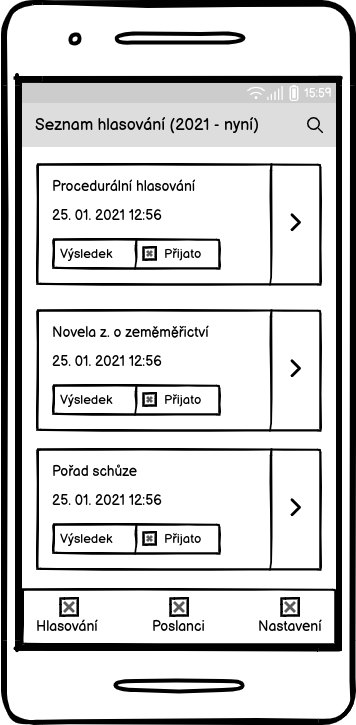
\includegraphics[scale = 0.5]{vote_list.png}
		\caption{Seznam hlasování}
		\label{fig:vote_list}
	\end{minipage}%
	\begin{minipage}{0.5\textwidth}
		\centering
		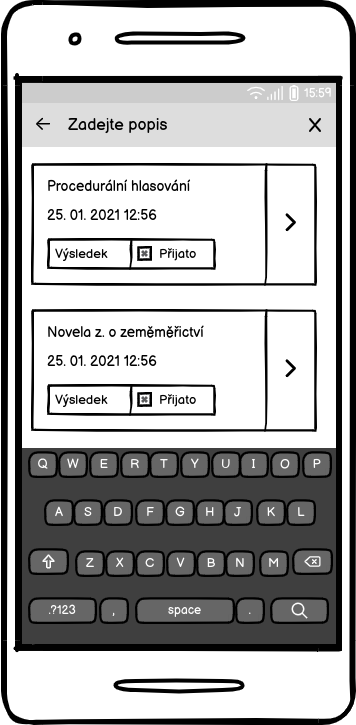
\includegraphics[scale = 0.5]{vote_list_search.png}
		\caption{Vyhledávání v seznamu hlasování}
		\label{fig:vote_list_search}
	\end{minipage}
\end{figure}

\begin{figure}[H]
	\begin{minipage}{0.5\textwidth}
		\centering
		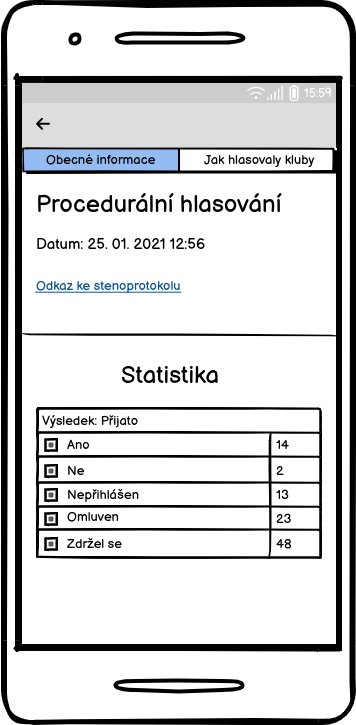
\includegraphics[scale = 0.4]{vote_details_general.png}
		\caption{Detail hlasování}
		\label{fig:vote_details_general}
	\end{minipage}%
	\begin{minipage}{0.5\textwidth}
		\centering
		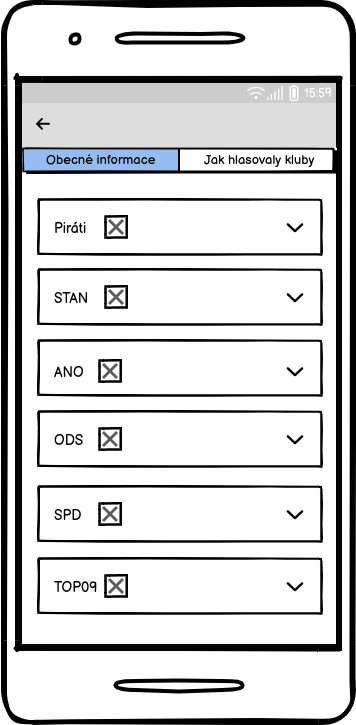
\includegraphics[scale = 0.4]{vote_details_party_votes.png}
		\caption{Jak hlasovaly kluby}
		\label{fig:vote_details_party_votes}
	\end{minipage}
	\begin{minipage}{0.5\textwidth}
		\centering
		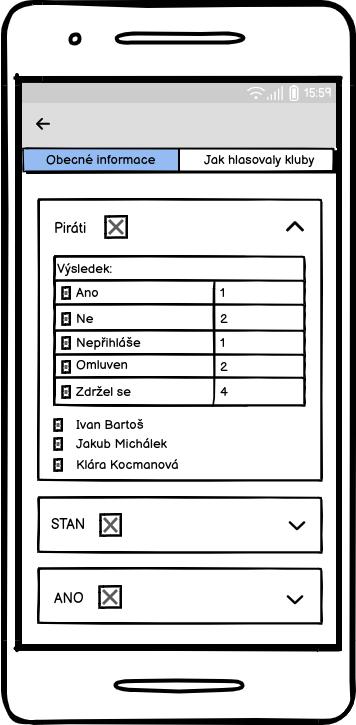
\includegraphics[scale = 0.4]{vote_details_party_votes_expanded.png}
		\caption{Jak hlasovaly kluby s expandovaným oknem klubu}
		\label{fig:vote_details_party_votes_expanded}
	\end{minipage}
\end{figure}

\begin{figure}[H]
	\begin{minipage}{0.5\textwidth}
		\centering
		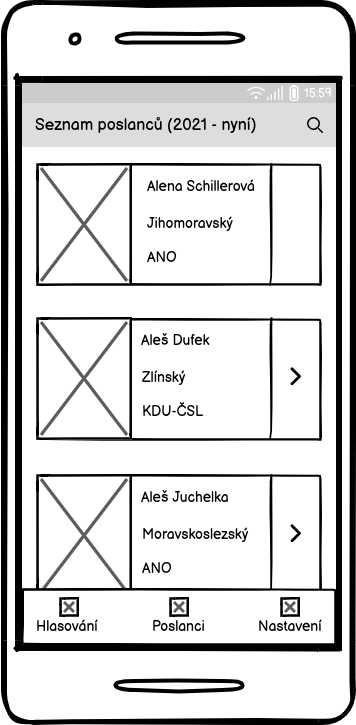
\includegraphics[scale = 0.5]{member_list.png}
		\caption{Seznam poslanců}
		\label{fig:member_list}
	\end{minipage}%
	\begin{minipage}{0.5\textwidth}
		\centering
		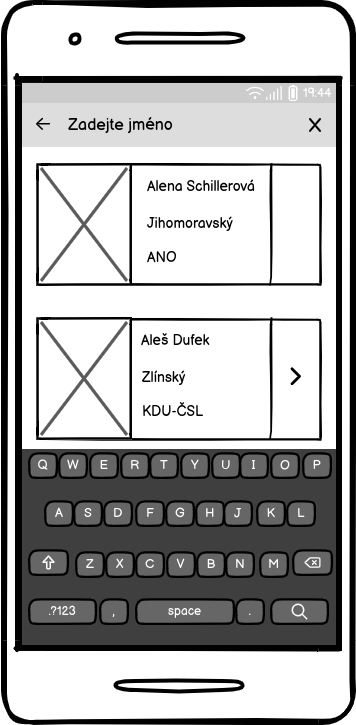
\includegraphics[scale = 0.5]{member_list_search.png}
		\caption{Vyhledávání v seznamu poslanců}
		\label{fig:member_list_search}
	\end{minipage}
\end{figure}

\begin{figure}[H]
	\begin{minipage}{0.5\textwidth}
		\centering
		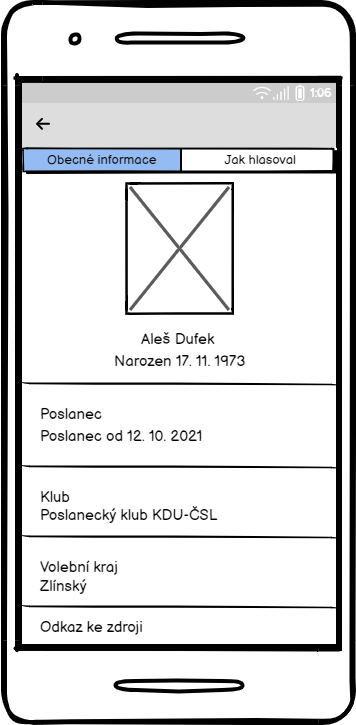
\includegraphics[scale = 0.5]{member_details_general.png}
		\caption{Detail poslance}
		\label{fig:member_details_general}
	\end{minipage}%
	\begin{minipage}{0.5\textwidth}
		\centering
		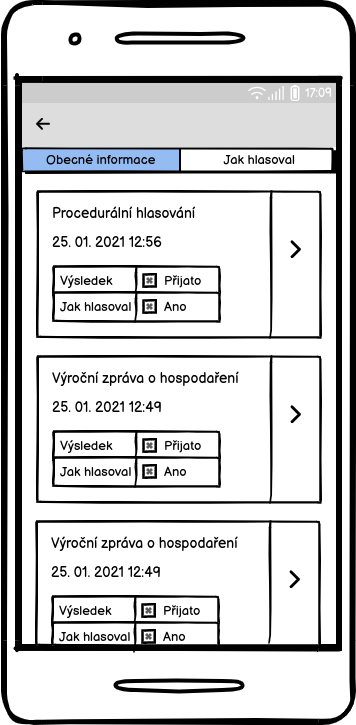
\includegraphics[scale = 0.5]{member_details_votes.png}
		\caption{Jak hlasoval poslanec}
		\label{fig:member_details_votes}
	\end{minipage}
\end{figure}

\begin{figure}[H]
	\begin{minipage}{0.5\textwidth}
		\centering
		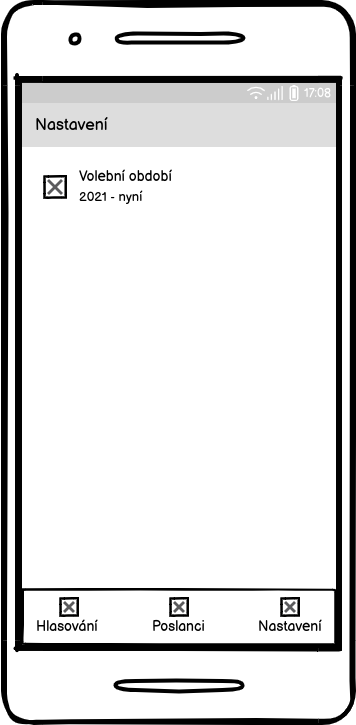
\includegraphics[scale = 0.5]{settings.png}
		\caption{Seznam nastavení}
		\label{fig:settings}
	\end{minipage}%
	\begin{minipage}{0.5\textwidth}
		\centering
		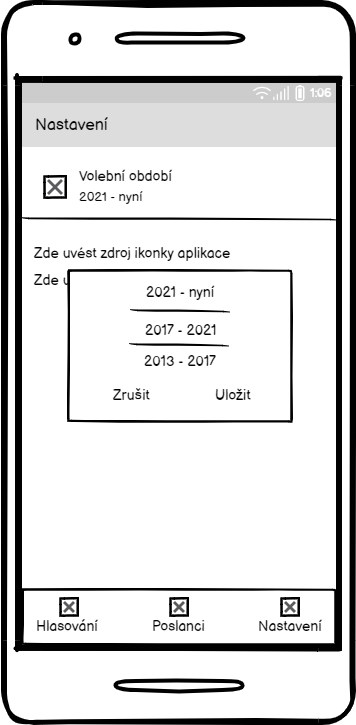
\includegraphics[scale = 0.5]{settings_opened.png}
		\caption{Nastavení volebního období}
		\label{fig:settings_opened}
	\end{minipage}
\end{figure} % include `appendix.tex' from `text/' subdirectory

\chapter{REST API odpovědi}


\begin{lstlisting}[caption={Tělo odpovědi pro dotaz \lstinline{GET /api/app}.}, label={fig:app}, language=json,firstnumber=1,tabsize=2]
	{
		"election_years": [
		2021,
		2017,
		2013,
		2010,
		2006,
		2002,
		1998,
		1996,
		1992
		]
	}
\end{lstlisting}

\begin{lstlisting}[caption={Tělo odpovědi pro dotaz \lstinline{GET /api/vote}}, label={fig:vote}, language=json,firstnumber=1,tabsize=2]
	[
	{
		"id": 1,
		"date_time": "16. 12. 2022 13:29",
		"description": "Hlasovani 1",
		"result": "A"
	},
	{
		"id": 2,
		"date_time": "16. 12. 2022 13:26",
		"description": "Hlasovani 2",
		"result": "A"
	},
	]
\end{lstlisting}

\begin{lstlisting}[caption={Tělo odpovědi pro dotaz \lstinline{GET /api/vote/{id}}}, label={fig:vote-1}, language=json,firstnumber=1,tabsize=2]
	{
		"id": 1,
		"date_time": "16. 12. 2022 13:29",
		"description": "Hlasovani 1,
		"result": "A",
		"steno_protocol_url": "http://www.psp.cz/eknih/2021ps/stenprot/048schuz",
		"source_url": "https://www.psp.cz/sqw/hlasy.sqw?g=77302&l=cz",
		"yes_count": 100,
		"no_count": 0,
		"logged_off_count": 64,
		"excused_count": 0,
		"refrained_count": 36,
		"election_year": 0
	}
\end{lstlisting}

\newpage

\begin{lstlisting}[caption={Tělo odpovědi pro dotaz \lstinline{GET /api/party/vote/1}}, label={fig:party-vote-1}, language=json,firstnumber=1,tabsize=2]
	[
	{
		"party_name": "Nazev klubu",
		"logo_url": "https://www.psp.cz/pics/klub/l-cps.jpg",
		"vote_id": 1,
		"party_results": {
			"yes_count": 2,
			"no_count": 0,
			"logged_off_count": 1,
			"excused_count": 0,
			"refrained_count": 0
		},
		"member_results": [
		{
			"member_name": "Poslanec 1",
			"vote_result": "@"
		},
		{
			"member_name": "Poslanec 2",
			"vote_result": "C"
		},
		{
			"member_name": "Poslanec 3",
			"vote_result": "A"
		},
		{
			"member_name": "Poslanec 4",
			"vote_result": "A"
		}
		]
	}
	]
\end{lstlisting}

\newpage

\begin{lstlisting}[caption={Tělo odpovědi pro dotaz \lstinline|GET /api/member|}, label={fig:member}, language=json,firstnumber=1,tabsize=2]
	[
	{
		"id": 1,
		"name": "Poslanec 1",
		"party": "ANO",
		"photo_url": "https://www.psp.cz/eknih/cdrom/2021ps/eknih/2021ps/poslanci/i6474.jpg",
		"election_region": "Volebni kraj 1",
		"election_year": 2021
	},
	{
		"id": 2,
		"name": "Poslanec 2",
		"party": "ODS",
		"photo_url": "https://www.psp.cz/eknih/cdrom/2021ps/eknih/2021ps/poslanci/i6804.jpg",
		"election_region": "Volebni kraj 2",
		"election_year": 2021
	},
	]
\end{lstlisting}

\begin{lstlisting}[caption={Tělo odpovědi pro dotaz \lstinline{GET /api/member/1}}, label={fig:member-1}, language=json,firstnumber=1,tabsize=2]
	{
		"id": 1,
		"name": "Poslanec 1",
		"gender": "M",
		"party": "Poslanecky klub",
		"member_from": "12. 10. 2021",
		"member_to": null,
		"date_of_birth": "25. 09. 1970",
		"election_region": "Volebni kraj 1",
		"photo_url": "https://www.psp.cz/eknih/cdrom/2021ps/eknih/2021ps/poslanci/i6474.jpg",
		"source_url": "https://www.psp.cz/sqw/detail.sqw?id=5700",
		"election_year": 2021
	}
\end{lstlisting}

\newpage

\begin{lstlisting}[caption={Tělo odpovědi pro dotaz \lstinline{GET /api/member/1/vote}}, label={fig:member-vote-1}, language=json,firstnumber=1,tabsize=2]
	[
	{
		"vote": {
			"id": 1,
			"date_time": "16. 12. 2022 13:29",
			"description": "Hlasovani 1",
			"result": "A"
		},
		"how_member_voted": "@"
	},
	{
		"vote": {
			"id": 2,
			"date_time": "16. 12. 2022 13:26",
			"description": "Hlasovani 2",
			"result": "A"
		},
		"how_member_voted": "@"
	}
	]
\end{lstlisting} % include `appendix.tex' from `text/' subdirectory

\chapter{Nějaká příloha}


Sem přijde to, co nepatří do hlavní části.
 % include `appendix.tex' from `text/' subdirectory

\backmatter % do not remove this command

\printbibliography % print out the BibLaTeX-generated bibliography list

\chapter{Obsah přiloženého média}


	\dirtree{%
		.1 readme.txt\DTcomment{stručný popis obsahu média}.
		.1 exe\DTcomment{adresář se spustitelnou formou implementace}.
		.1 src.
		.2 impl\DTcomment{zdrojové kódy implementace}.
		.2 thesis\DTcomment{zdrojová forma práce ve formátu \LaTeX{}}.
		.1 text\DTcomment{text práce}.
		.2 thesis.pdf\DTcomment{text práce ve formátu PDF}.
	}
 % include `medium.tex' from `text/' subdirectory

\end{document}
